\newpage
\chapter{HASIL DAN PEMBAHASAN} \label{Bab IV}

\section{Pengumpulan Data} \label{IV.Pengumpulan_Data}
Pada tahap ini dilakukan proses pengumpulan \textit{dataset} yang digunakan dalam penelitian. \textit{Dataset} yang digunakan adalah \textit{WildDeepfake}, yaitu \textit{dataset} publik untuk klasifikasi video \textit{deepfake} yang terdiri atas dua kelas, yaitu \textit{real} dan \textit{fake}. \textit{Dataset} ini digunakan sebagai sumber data utama dalam proses pelatihan, validasi, dan pengujian model.

\begin{table}[htbp]
	\centering
	\caption{Distribusi Kelas \textit{Dataset} \textit{WildDeepfake}}
	\label{table:4.wilddeepfake}
	\begin{tabular}{ccc}
		\toprule
		\textbf{Split} & \textbf{Kelas} & \textbf{Jumlah Video} \\
		\midrule
		\multirow{2}{*}{\textit{Train}} & \textit{Real} & 3.409 \\
		& \textit{Fake} & 3.099 \\
		\cmidrule(lr){1-3}
		\multirow{2}{*}{\textit{Test}} & \textit{Real} & 396 \\
		& \textit{Fake} & 410 \\
		\midrule
		\multicolumn{2}{c}{\textit{Total}} & 7.314 \\
		\bottomrule
	\end{tabular}
\end{table}

Berdasarkan Tabel \ref{table:4.wilddeepfake}, \textit{dataset} \textit{WildDeepfake} pada penelitian ini terdiri atas 6.508 video data latih dan 806 video data uji. Pada data latih, kelas \textit{real} berjumlah 3.409 video, sedangkan kelas \textit{fake} berjumlah 3.099 video. Pada data uji, kelas \textit{real} berjumlah 396 video, sedangkan kelas \textit{fake} berjumlah 410 video. Data tersebut selanjutnya diproses pada tahap \textit{pre-processing} untuk membentuk klip wajah yang digunakan sebagai masukan model.

\section{Hasil \textit{Pre-processing} Data} \label{IV.Preprocessing}
Tahap \textit{pre-processing} data dilakukan untuk menyiapkan \textit{dataset} \textit{WildDeepfake} agar dapat digunakan sebagai masukan model. Pada tahap ini, data yang sebelumnya berbentuk video wajah diproses menjadi klip dengan panjang seragam, kemudian dibagi ke dalam subset \textit{train}, validasi, dan \textit{test}.

\subsection{Hasil Pembentukan Klip 46 \textit{Frame}} \label{IV.Klip46}
Pada tahap ini, setiap video wajah pada \textit{dataset} \textit{WildDeepfake} diproses menjadi klip turunan dengan panjang tetap 46 \textit{frame}. Pembentukan klip dilakukan agar seluruh data memiliki panjang temporal yang seragam sebelum digunakan pada proses \textit{strided temporal sampling}. Dengan demikian, unit data yang digunakan pada tahap eksperimen bukan lagi video wajah awal, melainkan klip wajah berdurasi tetap.

Potongan kode yang digunakan untuk membentuk klip 46 \textit{frame} ditunjukkan pada Kode~\ref{code:4.1}.

\begin{lstlisting}[language=Python, caption={Pembentukan Klip 46 \textit{Frame}}, label={code:4.1}]
CLIP_LEN = 46

def compute_centered_clip_ranges(num_frames: int, clip_len: int = 46):
	"""
	Menghasilkan rentang [start, end) untuk klip 46 frame.
	Strategi:
	- C = floor(N / L)
	- R = N - C * L
	- buang floor(R/2) frame di kiri
	- buang ceil(R/2) frame di kanan
	"""
	if num_frames < clip_len:
		return []

	num_clips = num_frames // clip_len
	used_frames = num_clips * clip_len
	remainder = num_frames - used_frames

	discard_left = remainder // 2
	start_idx = discard_left

	ranges = []
	for i in range(num_clips):
		s = start_idx + i * clip_len
		e = s + clip_len
		ranges.append((s, e))

	return ranges

def build_46f_clips_for_subset(
	extracted_subset_dir: Path,
	processed_subset_dir: Path,
	clip_len: int = 46
):
	reset_dir(processed_subset_dir)

	group_dirs = sorted(
		[p for p in extracted_subset_dir.iterdir() if p.is_dir()],
		key=lambda p: p.name
	)

	total_videos = 0
	total_clips = 0
	skipped_videos = 0

	for group_dir in group_dirs:
		group_id = group_dir.name
		out_group_dir = processed_subset_dir / group_id
		ensure_dir(out_group_dir)

		video_dirs = sorted(
			[p for p in group_dir.iterdir() if p.is_dir()],
			key=lambda p: p.name
		)

		for video_dir in video_dirs:
			total_videos += 1
			video_id = video_dir.name

			frame_files = list_image_files(video_dir)
			n = len(frame_files)

			if n < clip_len:
				skipped_videos += 1
				continue

			clip_ranges = compute_centered_clip_ranges(n, clip_len=clip_len)

			for clip_idx, (s, e) in enumerate(clip_ranges):
				clip_folder_name = f"{video_id}_{clip_idx}"
				out_clip_dir = out_group_dir / clip_folder_name
				ensure_dir(out_clip_dir)

				selected_frames = frame_files[s:e]

				for frame_path in selected_frames:
					shutil.copy2(frame_path, out_clip_dir / frame_path.name)

				total_clips += 1

	return {
		"total_videos": total_videos,
		"total_clips": total_clips,
		"skipped_videos": skipped_videos,
	}
\end{lstlisting}

Kode~\ref{code:4.1} menunjukkan bahwa setiap video terlebih dahulu dihitung jumlah klip penuhnya berdasarkan panjang klip 46 \textit{frame}. Apabila terdapat sisa \textit{frame} yang tidak membentuk satu klip penuh, sisa tersebut dibuang dari sisi kiri dan kanan secara seimbang. Setelah itu, setiap rentang \textit{frame} disalin ke folder klip baru sehingga satu klip berisi tepat 46 \textit{frame}.

Pembentukan klip 46 \textit{frame} juga bertujuan agar \textit{frame} pada video yang lebih panjang tidak terlalu banyak terbuang. Karena model pada penelitian ini hanya membutuhkan 16 \textit{frame} sebagai masukan untuk satu klip, satu video yang memiliki ratusan \textit{frame} dapat dipecah menjadi beberapa klip turunan sebelum dilakukan \textit{strided temporal sampling}. Dengan strategi ini, informasi temporal dari satu video dapat dimanfaatkan secara lebih efisien dan jumlah data eksperimen yang dihasilkan menjadi lebih banyak.

Berdasarkan hasil pre-processing, diperoleh total 22.303 klip. Seluruh klip tersebut memiliki panjang 46 \textit{frame}, sehingga tidak terdapat klip yang tidak valid. Distribusi kelas hasil pembentukan klip 46 \textit{frame} ditunjukkan pada Tabel~\ref{table:4.klip46}.

\begin{table}[htbp]
	\centering
	\caption{Distribusi Kelas Hasil Pembentukan Klip 46 \textit{Frame}}
	\label{table:4.klip46}
	\begin{tabular}{|c|c|c|}
		\hline
		\textbf{Split} & \textbf{Kelas} & \textbf{Jumlah Klip} \\
		\hline
		\multirow{2}{*}{\textit{Train}} & \textit{Real} & 6.758 \\
		\cline{2-3}
		 & \textit{Fake} & 12.313 \\
		\hline
		\multirow{2}{*}{\textit{Test}} & \textit{Real} & 1.093 \\
		\cline{2-3}
		 & \textit{Fake} & 2.139 \\
		\hline
		\multicolumn{2}{|c|}{\textit{Total}} & 22.303 \\
		\hline
	\end{tabular}
\end{table}

Berdasarkan Tabel~\ref{table:4.klip46}, jumlah klip pada data latih terdiri atas 6.758 klip kelas \textit{real} dan 12.313 klip kelas \textit{fake}, sedangkan pada data uji terdiri atas 1.093 klip kelas \textit{real} dan 2.139 klip kelas \textit{fake}. Secara keseluruhan, hasil pembentukan klip menunjukkan bahwa distribusi data tetap didominasi oleh kelas \textit{fake} setelah video wajah diproses menjadi klip turunan.

\subsection{Hasil Pembagian \textit{Dataset}} \label{IV.Split}
\textit{Dataset} \textit{WildDeepfake} yang digunakan dalam penelitian ini sebelumnya telah memiliki pembagian awal berupa subset \textit{train} dan \textit{test}. Subset tersebut tersusun dalam empat direktori utama, yaitu \textit{real\_train}, \textit{fake\_train}, \textit{real\_test}, dan \textit{fake\_test}. Pada penelitian ini, subset \textit{real\_test} dan \textit{fake\_test} tetap digunakan sebagai data pengujian akhir. Sementara itu, data yang berasal dari subset \textit{real\_train} dan \textit{fake\_train} dibagi kembali menjadi data \textit{train} dan data validasi.

Pembagian data validasi dilakukan dari subset \textit{train} dengan rasio 80:20. Proses pembagian dilakukan pada level \textit{group\_id}, bukan pada level klip. Strategi ini digunakan agar klip turunan yang berasal dari video atau sumber yang sama tidak terpisah ke subset yang berbeda. Dengan demikian, risiko kebocoran data antara data latih dan data validasi dapat dikurangi.

Potongan kode pembagian \textit{dataset} ditunjukkan pada Kode~\ref{code:4.2}.

\begin{lstlisting}[language=Python, caption={Pembagian \textit{Dataset} \textit{Train}, Validasi, dan \textit{Test}}, label={code:4.2}]
SEED = 42
VAL_RATIO = 0.20

# Data train resmi berasal dari subset real_train dan fake_train.
train_records = []
train_records += build_manifest_for_subset("real_train", subset_dirs["real_train"])
train_records += build_manifest_for_subset("fake_train", subset_dirs["fake_train"])

# Data test resmi berasal dari subset real_test dan fake_test.
test_records = []
test_records += build_manifest_for_subset("real_test", subset_dirs["real_test"])
test_records += build_manifest_for_subset("fake_test", subset_dirs["fake_test"])

train_df = pd.DataFrame(train_records)
test_df = pd.DataFrame(test_records)

# Split dilakukan pada level GROUP, bukan level klip,
# agar klip turunan seperti 101_0, 101_1, dan 101_2
# tidak terpisah ke subset yang berbeda.
group_df = (
	train_df[["group_id", "label", "label_name"]]
	.drop_duplicates()
	.reset_index(drop=True)
)

train_groups, val_groups = train_test_split(
	group_df,
	test_size=VAL_RATIO,
	random_state=SEED,
	shuffle=True,
	stratify=group_df["label"],
)

train_group_ids = set(train_groups["group_id"])
val_group_ids = set(val_groups["group_id"])

train_split_df = (
	train_df[train_df["group_id"].isin(train_group_ids)]
	.copy()
	.reset_index(drop=True)
)

val_split_df = (
	train_df[train_df["group_id"].isin(val_group_ids)]
	.copy()
	.reset_index(drop=True)
)

test_df = test_df.reset_index(drop=True)

# Validasi anti-leakage antara train dan validasi.
overlap_groups = set(train_split_df["group_id"]) & set(val_split_df["group_id"])

if overlap_groups:
	raise ValueError(
		f"Ditemukan kebocoran group antara train dan validasi: "
		f"{list(overlap_groups)[:5]}"
	)
\end{lstlisting}

Kode~\ref{code:4.2} menunjukkan bahwa data uji tidak dibagi ulang, melainkan tetap mengikuti subset \textit{test} resmi dari \textit{dataset} \textit{WildDeepfake}. Pembagian ulang hanya dilakukan pada subset \textit{train} untuk membentuk data latih dan data validasi. Selain itu, penggunaan \textit{stratify=group\_df["label"]} bertujuan agar proporsi kelas \textit{real} dan \textit{fake} pada hasil pembagian tetap terjaga.

\begin{table}[htbp]
	\centering
	\caption{Hasil Pembagian \textit{Dataset} Berdasarkan Kelas}
	\label{table:4.split}
	\begin{tabular}{clrrr}
		\toprule
		\textbf{No} & \textbf{Subset} & \textbf{Real} & \textbf{Fake} & \textbf{Total} \\
		\midrule
		1 & \textit{Train} & 5.376 & 10.124 & 15.500 \\
		2 & Validasi & 1.382 & 2.189 & 3.571 \\
		3 & \textit{Test} & 1.093 & 2.139 & 3.232 \\
		\midrule
		\multicolumn{2}{l}{\textbf{Total}} & \textbf{7.851} & \textbf{14.452} & \textbf{22.303} \\
		\bottomrule
	\end{tabular}
\end{table}

Berdasarkan Tabel~\ref{table:4.split}, subset \textit{train} memiliki jumlah data terbesar, yaitu 15.500 klip. Subset validasi terdiri atas 3.571 klip, sedangkan subset \textit{test} terdiri atas 3.232 klip. Pada seluruh subset, jumlah klip kelas fake lebih banyak dibandingkan kelas real. Distribusi ini kemudian digunakan secara konsisten pada proses pelatihan, validasi, dan pengujian model.

\subsection{Augmentasi Data} \label{IV.Augmentasi}
Augmentasi data diterapkan untuk meningkatkan keragaman data pelatihan dan mengurangi risiko \textit{overfitting}. Pada penelitian ini, augmentasi hanya diterapkan pada subset \textit{train}, sedangkan subset validasi dan \textit{test} tidak diberikan augmentasi. Hal ini dilakukan agar proses validasi dan pengujian tetap merepresentasikan performa model pada data yang tidak mengalami transformasi tambahan.

Implementasi augmentasi dilakukan menggunakan library Albumentations. Library ini digunakan karena mendukung berbagai transformasi citra, seperti transformasi geometri, perubahan warna, blur, dan noise. Pada penelitian ini, augmentasi diterapkan secara konsisten pada seluruh \textit{frame} dalam satu klip. Dengan demikian, transformasi yang diberikan pada satu \textit{frame} direplikasi pada \textit{frame}-\textit{frame} lain dalam klip yang sama agar koherensi visual antar-\textit{frame} tetap terjaga.

Potongan kode augmentasi data ditunjukkan pada Kode~\ref{code:4.3}.

\begin{lstlisting}[language=Python, caption={Augmentasi Data Menggunakan Albumentations}, label={code:4.3}]
def _build_train_transform(self):
	crop_h, crop_w = _sample_fakeformer_crop_size(
		image_size=self.image_size,
		crop_limit=AUG_CROP_LIMIT,
	)

	return A.ReplayCompose(
		[
			A.OneOf(
				[
					A.RandomCrop(
						height=crop_h,
						width=crop_w,
						p=AUG_CROP_PROB,
					),
					A.RandomScale(
						scale_limit=AUG_SCALE_LIMIT,
						interpolation=cv2.INTER_LINEAR,
						p=AUG_SCALE_PROB,
					),
				],
				p=AUG_GEOMETRY_ONEOF_PROB,
			),
			A.Resize(
				height=self.image_size,
				width=self.image_size,
				interpolation=cv2.INTER_CUBIC,
				p=1.0,
			),
			A.HorizontalFlip(p=AUG_PROB_HFLIP),
			A.ColorJitter(
				brightness=AUG_COLORJITTER_BRIGHTNESS,
				contrast=AUG_COLORJITTER_CONTRAST,
				saturation=AUG_COLORJITTER_SATURATION,
				hue=AUG_COLORJITTER_HUE,
				p=AUG_COLORJITTER_PROB,
			),
			A.OneOf(
				[
					A.GaussianBlur(
						blur_limit=AUG_GAUSSIAN_BLUR_LIMIT,
						sigma_limit=0,
						p=AUG_GAUSSIAN_BLUR_PROB,
					),
					_make_gauss_noise_transform(
						p=AUG_GAUSSNOISE_PROB,
					),
				],
				p=AUG_BLUR_OR_NOISE_ONEOF_PROB,
			),
		]
	)
\end{lstlisting}

Kode~\ref{code:4.3} menunjukkan bahwa augmentasi yang digunakan terdiri atas beberapa jenis transformasi, yaitu random crop, random scale, horizontal flip, color jitter, Gaussian blur, dan Gaussian noise. Transformasi random crop dan random scale digunakan untuk memberikan variasi geometri pada area wajah. Transformasi horizontal flip digunakan untuk menambah variasi orientasi wajah. Transformasi color jitter digunakan untuk mensimulasikan variasi pencahayaan dan warna. Sementara itu, Gaussian blur dan Gaussian noise digunakan untuk menambahkan variasi degradasi visual yang dapat muncul pada data video.

Contoh visualisasi hasil augmentasi ditunjukkan pada Gambar~\ref{fig:4.augmentasi}. Visualisasi tersebut menampilkan perbandingan antara citra asli dan beberapa hasil augmentasi yang diterapkan pada data latih.

\begin{figure}[htbp]
	\centering
	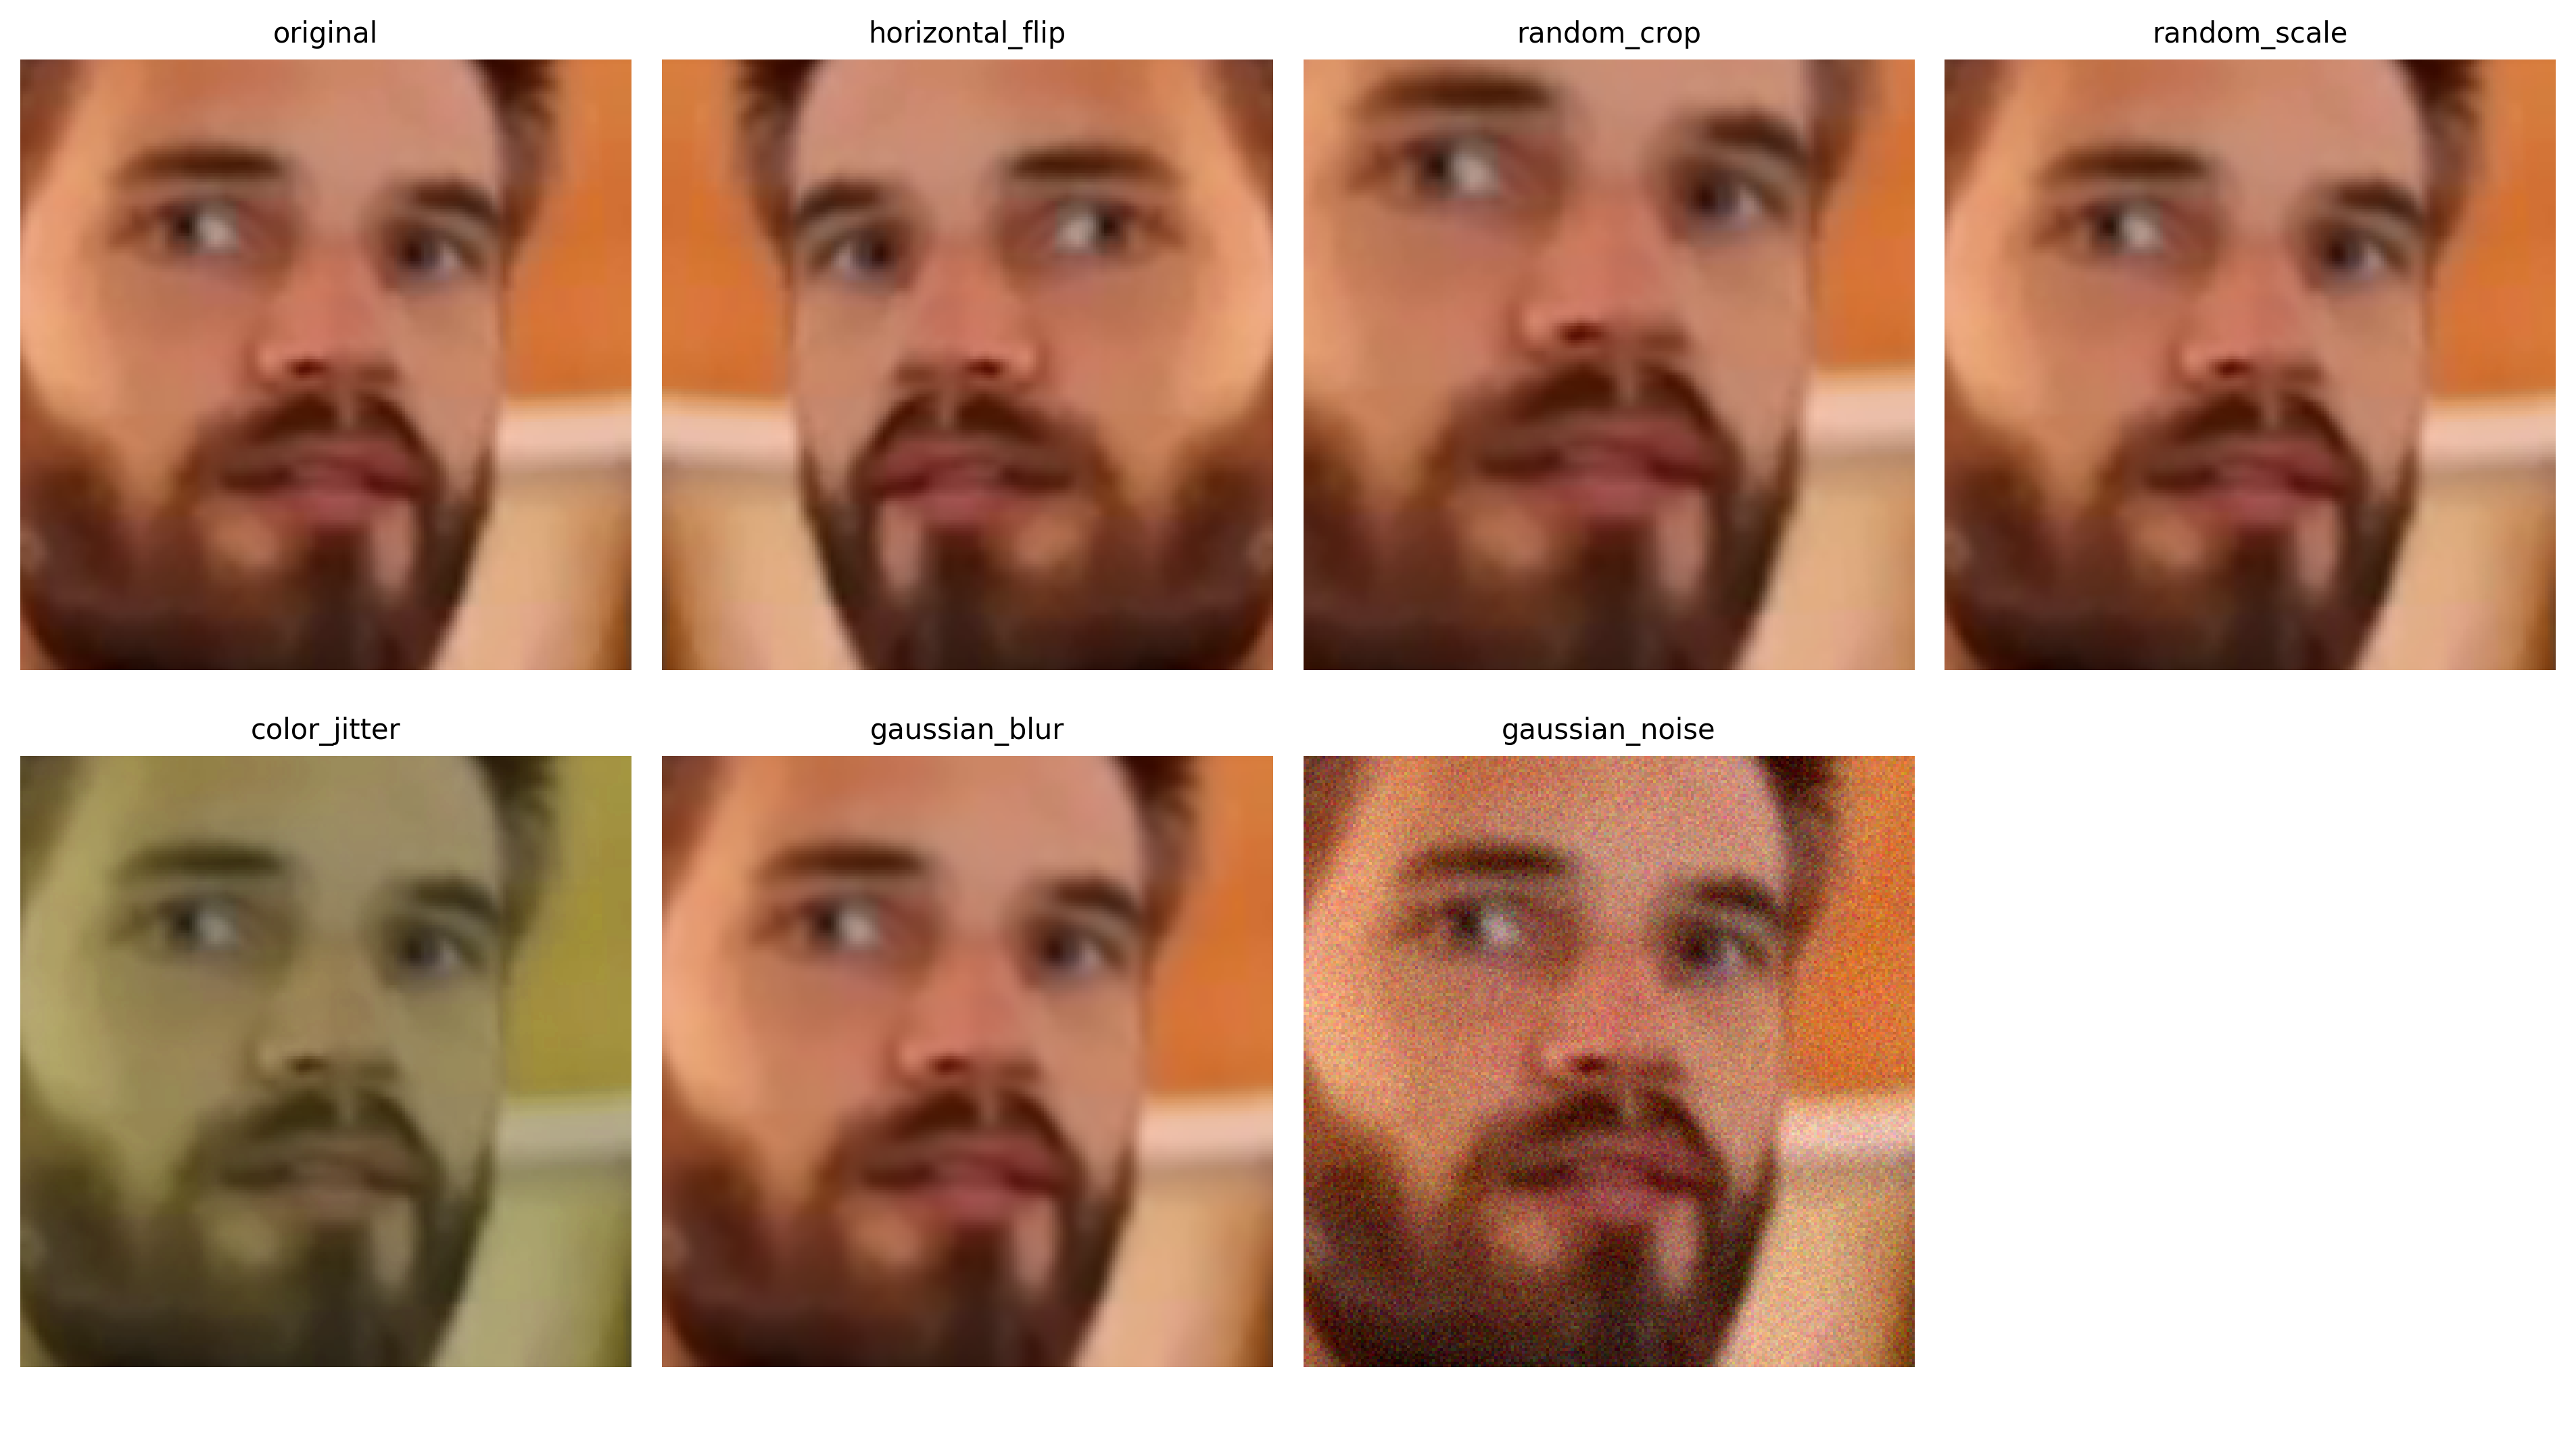
\includegraphics[width=1.1\textwidth]{figure/augmentation_grid.png}
	\caption{Contoh Hasil Augmentasi Data Menggunakan Albumentations: (a) citra asli, (b) horizontal flip, (c) random crop, (d) random scale, (e) color jitter, (f) Gaussian blur, dan (g) Gaussian noise}
	\label{fig:4.augmentasi}
\end{figure}

Berdasarkan Gambar~\ref{fig:4.augmentasi}, augmentasi yang diterapkan tidak mengubah label data, tetapi hanya memberikan variasi visual pada citra wajah. Dengan demikian, model diharapkan dapat mempelajari pola yang lebih robust terhadap perubahan posisi wajah, orientasi, pencahayaan, serta degradasi visual pada \textit{frame}.

\subsection{Normalisasi Data} \label{IV.Normalisasi}
Setelah proses augmentasi dilakukan, setiap \textit{frame} dikonversi menjadi \textit{tensor} dan dinormalisasi sebelum diberikan ke model. Normalisasi dilakukan untuk menyesuaikan distribusi nilai piksel dengan karakteristik model \textit{pretrained} yang digunakan. Pada penelitian ini, nilai piksel terlebih dahulu diubah ke rentang [0, 1], kemudian dinormalisasi menggunakan nilai mean dan standard deviation ImageNet.

Potongan kode normalisasi data ditunjukkan pada Kode~\ref{code:4.4}.

\begin{lstlisting}[language=Python, caption={Normalisasi Data}, label={code:4.4}]
NORM_MEAN = (0.485, 0.456, 0.406)
NORM_STD = (0.229, 0.224, 0.225)

def _array_to_normalized_tensor(self, image_array: np.ndarray):
	tensor = torch.from_numpy(image_array).permute(2, 0, 1).float()

	if image_array.dtype == np.uint8:
		tensor = tensor / 255.0
	elif tensor.max() > 1.0:
		tensor = tensor / 255.0

	tensor = torch.clamp(tensor, 0.0, 1.0)

	tensor = TF.normalize(
		tensor,
		mean=self.mean,
		std=self.std,
	)

	return tensor
\end{lstlisting}

Kode~\ref{code:4.4} menunjukkan bahwa citra yang semula berada dalam format H $\times$ W $\times$ C dikonversi menjadi format \textit{tensor} C $\times$ H $\times$ W. Selanjutnya, nilai piksel dikonversi ke rentang [0, 1] dengan membagi nilai piksel 8-bit terhadap 255. Setelah itu, normalisasi dilakukan menggunakan nilai mean (0,485, 0,456, 0,406) dan standard deviation (0,229, 0,224, 0,225).

Normalisasi diterapkan pada seluruh subset data, yaitu \textit{train}, validasi, dan \textit{test}. Perbedaannya adalah subset \textit{train} terlebih dahulu melalui proses augmentasi, sedangkan subset validasi dan \textit{test} hanya melalui proses transformasi dasar, konversi \textit{tensor}, dan normalisasi. Dengan demikian, seluruh data yang diberikan ke model memiliki format dan skala nilai yang konsisten pada tahap pelatihan, validasi, dan pengujian.

\section{Hasil Rancangan Model} \label{IV.Model}
Tahap rancangan model dilakukan untuk mengimplementasikan dua pendekatan klasifikasi video \textit{deepfake}, yaitu pendekatan spasial dan pendekatan spasiotemporal. Kedua pendekatan menggunakan data masukan yang berasal dari hasil \textit{strided temporal sampling} yang sama, sehingga perbandingan performa dapat dilakukan secara lebih setara. Perbedaan utama kedua model terletak pada cara model memproses \textit{frame} dalam satu klip. Model spasial memproses \textit{frame} secara individual, sedangkan model spasiotemporal memproses seluruh \textit{frame} dalam satu klip secara langsung.

\subsection{Model Spasial} \label{IV.Model_Spasial}
Model spasial pada penelitian ini menggunakan arsitektur \textit{Vision Transformer} (ViT). Model ini dirancang untuk memproses informasi visual pada tingkat \textit{frame}. Oleh karena itu, meskipun data dari dataloader berbentuk klip, setiap \textit{frame} dalam klip tetap diperlakukan sebagai citra individual sebelum diberikan ke model.

Pada implementasinya, satu \textit{batch} data memiliki bentuk \textit{tensor} $B \times T \times C \times H \times W$, dengan $B$ sebagai ukuran \textit{batch}, $T$ sebagai jumlah \textit{frame} dalam satu klip, $C$ sebagai jumlah kanal warna, serta $H$ dan $W$ sebagai tinggi dan lebar citra. Karena ViT menerima input berupa citra, \textit{tensor} klip yang semula berbentuk $B \times T \times C \times H \times W$ terlebih dahulu diubah menjadi bentuk $(B \times T) \times C \times H \times W$ dengan menggabungkan dimensi \textit{batch} dan temporal. Dengan demikian, seluruh \textit{frame} dalam \textit{batch} dapat diproses sebagai kumpulan citra tunggal oleh ViT.

Setelah model menghasilkan \textit{logit} untuk setiap \textit{frame}, \textit{logit} tersebut dikembalikan ke bentuk $B \times T \times 2$. Angka 2 menunjukkan jumlah kelas klasifikasi, yaitu \textit{real} dan \textit{fake}. Selanjutnya, \textit{logit} dari seluruh \textit{frame} dalam satu klip dirata-ratakan pada dimensi temporal untuk menghasilkan satu prediksi akhir pada tingkat klip. Potongan kode implementasi model spasial ditunjukkan pada Kode~\ref{code:4.5}.

\begin{lstlisting}[language=Python, caption={Implementasi Model Spasial}, label={code:4.5}]
b, t, c, h, w = clips.shape

clips = clips.to(device, non_blocking=True)
labels = labels.to(device, non_blocking=True)

frames = clips.reshape(b * t, c, h, w)

with torch.autocast(device_type=DEVICE.type, dtype=AMP_DTYPE, enabled=USE_AMP):
	frame_logits = model(frames)
	clip_logits = frame_logits.view(b, t, 2).mean(dim=1)
	loss = criterion(clip_logits, labels)
\end{lstlisting}

Kode~\ref{code:4.5} menunjukkan bahwa model spasial tidak memproses video secara langsung, melainkan memproses setiap \textit{frame} sebagai citra individual. Proses \textit{reshape} digunakan untuk menggabungkan dimensi \textit{batch} dan dimensi temporal, sehingga input yang diterima ViT berbentuk kumpulan \textit{frame}. Setelah \textit{logit} setiap \textit{frame} diperoleh, hasil tersebut diagregasi menggunakan rata-rata untuk memperoleh \textit{logit} tingkat klip.

Melalui mekanisme ini, model spasial tetap mempertahankan karakteristik sebagai model berbasis citra, tetapi hasil akhirnya tetap berada pada tingkat klip. Hal ini diperlukan agar hasil evaluasi model spasial dapat dibandingkan secara langsung dengan model spasiotemporal. Dengan demikian, model spasial digunakan untuk mengukur sejauh mana informasi visual statis pada \textit{frame} mampu membedakan klip \textit{real} dan \textit{fake}.

\subsection{Model Spasiotemporal} \label{IV.Model_Spasiotemporal}
Model spasiotemporal pada penelitian ini menggunakan arsitektur \textit{VideoMAE}. Berbeda dengan model spasial, model ini dirancang untuk menerima masukan berupa klip video secara langsung. Oleh karena itu, hubungan antar-\textit{frame} dalam satu klip tetap dipertahankan selama proses pemodelan.

Pada implementasinya, data dari dataloader memiliki bentuk \textit{tensor} $B \times T \times C \times H \times W$. Bentuk tersebut tidak diubah menjadi kumpulan \textit{frame} individual, melainkan langsung diberikan ke model \textit{VideoMAE} melalui parameter \texttt{pixel\_values}. Dengan rancangan ini, model dapat mempelajari informasi spasial pada setiap \textit{frame} sekaligus hubungan temporal antar-\textit{frame} dalam satu klip.

Model \textit{VideoMAE} menghasilkan \textit{logit} secara langsung pada tingkat klip. Oleh karena itu, tidak diperlukan proses agregasi \textit{logit} antar-\textit{frame} seperti pada model spasial. Potongan kode implementasi model spasiotemporal ditunjukkan pada Kode~\ref{code:4.6}.

\begin{lstlisting}[language=Python, caption={Implementasi Model Spasiotemporal}, label={code:4.6}]
clips = clips.to(device, non_blocking=True)
labels = labels.to(device, non_blocking=True)

optimizer.zero_grad(set_to_none=True)

with torch.autocast(device_type=device.type, dtype=AMP_DTYPE, enabled=USE_AMP):
	outputs = model(pixel_values=clips)
	logits = outputs.logits
	loss = criterion(logits, labels)
\end{lstlisting}

Kode~\ref{code:4.6} menunjukkan bahwa model spasiotemporal menerima input klip secara langsung dalam bentuk $B \times T \times C \times H \times W$. Variabel \texttt{clips} merepresentasikan \textit{batch} klip hasil sampling yang telah melalui proses normalisasi. Selanjutnya, klip tersebut diberikan ke \textit{VideoMAE} melalui \texttt{model(pixel\_values=clips)}, kemudian model menghasilkan \textit{logit} untuk dua kelas, yaitu \textit{real} dan \textit{fake}.

Dengan mekanisme tersebut, model spasiotemporal dapat memanfaatkan informasi visual pada setiap \textit{frame} sekaligus pola perubahan antar-\textit{frame} dalam satu klip. Pendekatan ini berbeda dari model spasial yang hanya memproses \textit{frame} secara individual. Oleh karena itu, model spasiotemporal digunakan untuk mengevaluasi apakah pemodelan temporal dapat memberikan kontribusi terhadap peningkatan performa klasifikasi video \textit{deepfake} pada \textit{dataset} \textit{WildDeepfake}.

\subsection{Konfigurasi \textit{Hyperparameter}} \label{IV.Hyperparameter}
Konfigurasi \textit{hyperparameter} digunakan untuk mengatur proses pelatihan model pada eksperimen \textit{baseline}. \textit{Hyperparameter} ini diterapkan untuk membangun konfigurasi awal sebelum dilakukan variasi eksperimen lebih lanjut. Pemilihan konfigurasi \textit{baseline} mengacu pada penelitian Nguyen et al. \cite{nguyen2024fakeformerefficientvulnerabilitydriventransformers} yang menggunakan pendekatan berbasis \textit{Transformer} untuk deteksi \textit{deepfake}. Konfigurasi tersebut kemudian disesuaikan dengan rancangan eksperimen, ketersediaan sumber daya komputasi, serta kebutuhan perbandingan yang setara antara model spasial berbasis ViT dan model spasiotemporal berbasis \textit{VideoMAE}.

\begin{table}[htbp]
	\centering
	\caption{Hyperparameter Model Baseline}
	\label{table:4.hyperparam}
	\begin{tabular}{cll}
		\toprule
		\textbf{No} & \textbf{Parameter} & \textbf{Nilai} \\
		\midrule
		1 & \textit{Learning rate} & $5\times10^{-5}$ \\
		2 & \textit{Batch size} & 32 \\
		3 & Epoch maksimum & 25 \\
		4 & \textit{Optimizer} & AdamW \\
		5 & \textit{Weight decay} & $1\times10^{-4}$ \\
		6 & \textit{Scheduler} & \textit{Linear Decay LR} \\
		7 & \textit{Loss function} & CrossEntropyLoss \\
		8 & \textit{Dropout} & 0 \\
		\bottomrule
	\end{tabular}
\end{table}

Berdasarkan Tabel~\ref{table:4.hyperparam}, model \textit{baseline} dilatih menggunakan \textit{learning rate} sebesar $5\times10^{-5}$ dengan \textit{epoch} maksimum sebanyak 25 \textit{epoch}. \textit{Optimizer} yang digunakan adalah AdamW dengan \textit{weight decay} sebesar $1\times10^{-4}$. Penggunaan \textit{weight decay} bertujuan untuk memberikan regularisasi pada bobot model selama proses pelatihan. \textit{Scheduler} yang digunakan adalah \textit{Linear Decay LR}, yaitu penurunan \textit{learning rate} secara bertahap hingga mendekati nol selama proses pelatihan.

Fungsi \textit{loss} yang digunakan adalah CrossEntropyLoss karena penelitian ini merupakan tugas klasifikasi biner dengan dua kelas, yaitu \textit{real} dan \textit{fake}. Nilai \textit{dropout} ditetapkan sebesar 0, sehingga tidak terdapat penambahan \textit{dropout} khusus pada konfigurasi \textit{baseline}. Dengan konfigurasi ini, model \textit{baseline} digunakan sebagai acuan awal untuk mengevaluasi performa pendekatan spasial dan spasiotemporal sebelum dibandingkan dengan konfigurasi eksperimen lainnya.

\section{Hasil Eksperimen} \label{IV.Eksperimen}
Pada sub bab ini, hasil eksperimen disajikan dalam empat subbab utama. Pertama, hasil eksperimen \textit{baseline} digunakan sebagai acuan awal performa model. Kedua, hasil konfigurasi pelatihan digunakan untuk menganalisis pengaruh perubahan parameter pelatihan terhadap performa model. Ketiga, hasil konfigurasi input spasial dan temporal digunakan untuk mengevaluasi pengaruh perubahan resolusi, jumlah \textit{frame}, dan \textit{stride} terhadap pendekatan spasial dan spasiotemporal. Keempat, evaluasi lintas-\textit{dataset} digunakan untuk menguji kemampuan generalisasi model pada \textit{dataset} eksternal secara \textit{zero-shot}.

\subsection{Hasil Eksperimen \textit{Baseline}} \label{IV.Eksperimen_Baseline}
Eksperimen \textit{baseline} dilakukan untuk memperoleh gambaran performa awal dari pendekatan spasial dan spasiotemporal sebelum dilakukan variasi konfigurasi pada tahap eksperimen berikutnya. Pada eksperimen ini, kedua model menggunakan konfigurasi dasar, yaitu resolusi input 224 $\times$ 224 piksel, jumlah \textit{frame} masukan sebanyak 16 \textit{frame}, dan nilai \textit{stride} sebesar 3. Model spasial menggunakan \textit{Vision Transformer} untuk memproses \textit{frame} secara individual, sedangkan model spasiotemporal menggunakan \textit{VideoMAE} untuk memproses klip video secara langsung.

\begin{table}[htbp]
	\centering
	\caption{Hasil Eksperimen \textit{Baseline}}
	\label{table:4.baseline}
	\begin{tabular}{lccccc}
		\toprule
		\textbf{Kode} &
		\textbf{\textit{Acc}} &
		\textbf{\textit{Prec}} &
		\textbf{\textit{Rec}} &
		\textbf{\textit{F1}} &
		\textbf{\textit{AUC}} \\
		\midrule
			BASE-SP & 79,2\% & 76,8\% & 76,7\% & 76,7\% & 86,8\% \\
			BASE-ST & \textbf{85,8\%} & \textbf{83,9\%} & \textbf{85,5\%} & \textbf{84,5\%} & \textbf{92,3\%} \\
		\bottomrule
	\end{tabular}
\end{table}

Berdasarkan Tabel~\ref{table:4.baseline}, model spasiotemporal BASE-ST memperoleh performa yang lebih tinggi dibandingkan model spasial BASE-SP pada seluruh metrik evaluasi. Pada metrik \textit{accuracy}, model spasiotemporal mencapai nilai sebesar 85,8\%, sedangkan model spasial mencapai 79,2\%. Pada metrik \textit{F1}, model spasiotemporal memperoleh nilai 84,5\%, lebih tinggi dibandingkan model spasial sebesar 76,7\%. Demikian pula pada metrik \textit{AUC}, model spasiotemporal memperoleh nilai 92,3\%, sedangkan model spasial memperoleh 86,8\%. Hasil ini menunjukkan bahwa pada konfigurasi \textit{baseline}, pendekatan spasiotemporal memiliki kemampuan klasifikasi dan kemampuan diskriminasi kelas yang lebih baik dibandingkan pendekatan spasial.

\begin{figure}[htbp]
	\centering
	\begin{minipage}{0.65\textwidth}
		\centering
		
\includegraphics[width=\textwidth]{\detokenize{figure/Hasil Eksperimen/Eksperimen Utama 1 Baseline/Model Spasial/Loss.png}}
		\\(a) Model spasial
	\end{minipage}
	
	\vspace{0.75em}
	
	\begin{minipage}{0.65\textwidth}
		\centering
		
\includegraphics[width=\textwidth]{\detokenize{figure/Hasil Eksperimen/Eksperimen Utama 1 Baseline/Model Spasiotemporal/Loss.png}}
		\\(b) Model spasiotemporal
	\end{minipage}
	\caption{Kurva \textit{training loss} dan \textit{validation loss} pada eksperimen \textit{baseline}.}
	\label{fig:4.baseline-loss}
\end{figure}

Berdasarkan Gambar~\ref{fig:4.baseline-loss}, kurva \textit{training loss} pada model spasial dan spasiotemporal sama-sama menurun secara bertahap selama proses pelatihan. Pola ini menunjukkan bahwa kedua model mampu mempelajari pola dari data latih dengan baik. Sementara itu, \textit{validation loss} pada kedua model masih menunjukkan fluktuasi pada beberapa \textit{epoch}, tetapi tidak mengalami peningkatan secara terus-menerus. Hal ini mengindikasikan bahwa proses pelatihan masih berjalan stabil dan tidak menunjukkan gejala \textit{overfitting} yang berat pada konfigurasi \textit{baseline}.

Jika dibandingkan, model spasiotemporal menunjukkan nilai \textit{validation loss} akhir yang lebih rendah dibandingkan model spasial. Kondisi ini menunjukkan bahwa model spasiotemporal memiliki kemampuan generalisasi yang lebih baik terhadap data validasi. Temuan tersebut sejalan dengan hasil evaluasi pada data uji, yaitu model spasiotemporal memperoleh performa yang lebih tinggi dibandingkan model spasial.

\begin{figure}[htbp]
	\centering
	\begin{minipage}{0.65\textwidth}
		\centering
		
\includegraphics[width=\textwidth]{\detokenize{figure/Hasil Eksperimen/Eksperimen Utama 1 Baseline/Model Spasial/Accuracy.png}}
		\\(a) Model spasial
	\end{minipage}
	
	\vspace{0.75em}
	
	\begin{minipage}{0.65\textwidth}
		\centering
		
\includegraphics[width=\textwidth]{\detokenize{figure/Hasil Eksperimen/Eksperimen Utama 1 Baseline/Model Spasiotemporal/Accuracy.png}}
		\\(b) Model spasiotemporal
	\end{minipage}
	\caption{Kurva \textit{training accuracy} dan \textit{validation accuracy} pada eksperimen \textit{baseline}.}
	\label{fig:4.baseline-acc}
\end{figure}

Berdasarkan Gambar~\ref{fig:4.baseline-acc}, kurva \textit{training accuracy} pada kedua model menunjukkan peningkatan secara bertahap dari awal hingga akhir pelatihan. \textit{validation accuracy} juga memperlihatkan tren peningkatan dan cenderung stabil pada \textit{epoch} akhir. Hal ini menunjukkan bahwa kedua model mampu meningkatkan kemampuan klasifikasi selama proses pelatihan.

Namun, model spasiotemporal menghasilkan \textit{validation accuracy} yang lebih tinggi dibandingkan model spasial. Dengan demikian, kurva \textit{accuracy} memperkuat hasil pada Tabel~\ref{table:4.baseline} bahwa pendekatan spasiotemporal memiliki performa pembelajaran dan generalisasi yang lebih baik pada eksperimen \textit{baseline}. Secara keseluruhan, pola kurva \textit{loss} dan \textit{accuracy} menunjukkan bahwa kedua model berhasil dilatih dengan stabil, tetapi model spasiotemporal memberikan hasil yang lebih unggul.

\begin{figure}[htbp]
	\centering
	\begin{minipage}{0.48\textwidth}
		\centering
		
\includegraphics[width=\textwidth]{\detokenize{figure/Hasil Eksperimen/Eksperimen Utama 1 Baseline/Model Spasial/confusion-matrix.png}}
		\\(a) Model spasial
	\end{minipage}
	\hfill
	\begin{minipage}{0.48\textwidth}
		\centering
		
\includegraphics[width=\textwidth]{\detokenize{figure/Hasil Eksperimen/Eksperimen Utama 1 Baseline/Model Spasiotemporal/confusion-matrix.png}}
		\\(b) Model spasiotemporal
	\end{minipage}
	\caption{\textit{Confusion matrix} pada eksperimen \textit{baseline}.}
	\label{fig:4.baseline-cm}
\end{figure}


Berdasarkan \textit{confusion matrix} pada Gambar~\ref{fig:4.baseline-cm}, jumlah \textit{false positive} dan \textit{false negative} pada model spasial masih relatif tinggi. \textit{False positive} menunjukkan bahwa sebagian data \textit{real} masih keliru diklasifikasikan sebagai \textit{fake}. Kondisi ini mengindikasikan bahwa model spasial cenderung sensitif terhadap karakteristik visual tertentu yang dianggap menyerupai artefak manipulasi. Akibatnya, sebagian video \textit{real} dengan variasi pencahayaan, pose, kompresi, atau kualitas visual tertentu dapat salah dikenali sebagai \textit{fake}. Sementara itu, \textit{false negative} menunjukkan bahwa sebagian data \textit{fake} belum berhasil terdeteksi dan masih diklasifikasikan sebagai \textit{real}. Hal ini memperlihatkan keterbatasan pendekatan spasial dalam menangkap klip \textit{fake} yang artefak manipulasinya tidak cukup jelas pada tingkat \textit{frame} individual.

Pada model spasiotemporal, jumlah \textit{false positive} lebih rendah dibandingkan model spasial. Penurunan \textit{false positive} ini menunjukkan bahwa \textit{VideoMAE} lebih mampu membedakan variasi visual alami pada video \textit{real} dari pola manipulasi pada video \textit{fake}. Dengan kata lain, model spasiotemporal lebih jarang memberikan prediksi \textit{fake} terhadap data yang sebenarnya \textit{real}. Hal ini penting karena \textit{false positive} yang tinggi dapat menyebabkan video asli keliru dianggap sebagai \textit{deepfake} \cite{Gu2021}\cite{Haliassos2021}.

Selain itu, model spasiotemporal juga menghasilkan \textit{false negative} yang lebih rendah dibandingkan model spasial, meskipun penurunannya tidak sebesar penurunan \textit{false positive}. Hal ini menunjukkan bahwa pemanfaatan informasi temporal antar-\textit{frame} membantu model dalam mendeteksi sebagian klip \textit{fake} yang tidak cukup kuat apabila hanya dianalisis melalui informasi spasial pada \textit{frame} tunggal. Namun, masih adanya \textit{false negative} menunjukkan bahwa beberapa klip \textit{fake} tetap sulit dikenali, terutama apabila pola manipulasinya halus atau tidak konsisten sepanjang \textit{frame} \cite{Gu2021}\cite{tong2022videomaemaskedautoencodersdataefficient}.

Jika dibandingkan, peningkatan utama model spasiotemporal terlihat pada kemampuannya menekan \textit{false positive} secara lebih besar dibandingkan model spasial. Artinya, keunggulan \textit{VideoMAE} pada eksperimen \textit{baseline} tidak hanya berasal dari peningkatan kemampuan mendeteksi kelas \textit{fake}, tetapi juga dari peningkatan kemampuan mempertahankan data \textit{real} agar tidak salah diklasifikasikan sebagai \textit{fake}. Pola ini sejalan dengan nilai \textit{accuracy}, \textit{F1}, dan \textit{AUC} yang lebih tinggi pada model spasiotemporal \cite{Gu2021}\cite{KINGRA2024301817}\cite{tong2022videomaemaskedautoencodersdataefficient}.

Secara keseluruhan, hasil eksperimen \textit{baseline} menunjukkan bahwa model spasiotemporal memberikan performa yang lebih baik dibandingkan model spasial. Keunggulan tersebut terlihat dari nilai metrik evaluasi yang lebih tinggi, pola kurva pelatihan yang lebih stabil, serta jumlah kesalahan klasifikasi yang lebih rendah pada \textit{confusion matrix}. Oleh karena itu, hasil \textit{baseline} ini digunakan sebagai acuan awal untuk menilai pengaruh perubahan konfigurasi pada tahap pengujian konfigurasi pelatihan.

\subsection{Hasil Konfigurasi Pelatihan} \label{IV.Eksperimen_Ablation}
Pengujian konfigurasi pelatihan dilakukan untuk menganalisis pengaruh perubahan satu komponen pelatihan terhadap performa model spasial dan spasiotemporal. Pada setiap eksperimen, satu parameter diubah dari konfigurasi \textit{baseline}, sedangkan parameter lainnya dipertahankan tetap. Dengan demikian, perubahan performa dapat dianalisis secara lebih terarah berdasarkan parameter yang diuji.

Setiap hasil konfigurasi pelatihan dibandingkan langsung dengan \textit{baseline} BASE-SP dan BASE-ST. Model BASE-SP digunakan sebagai acuan pendekatan spasial, sedangkan BASE-ST digunakan sebagai acuan pendekatan spasiotemporal. Pembahasan disusun secara bertahap, dimulai dari pengaruh \textit{epoch} maksimum, \textit{learning rate}, \textit{loss function}, augmentasi data, \textit{dropout}, hingga \textit{scheduler}. Pada setiap subbab, analisis difokuskan pada tujuan perubahan konfigurasi, alasan pemilihan nilai parameter, serta dampaknya terhadap metrik evaluasi model.

\begin{table}[htbp]
\centering
\caption{Konfigurasi Pelatihan yang Diuji}
\label{table:4.ablation-config}
\begin{tabular}{llll}
\toprule
\textbf{Kode} &
\textbf{Parameter} &
\textbf{Nilai \textit{Baseline}} &
\textbf{Nilai Uji} \\
\midrule
M1 & \textit{Epoch} & 25 \textit{epoch} & 40 \textit{epoch} \\
M2 & \textit{Learning rate} & 5e-5 & 5e-4 \\
M3 & \textit{Loss function} & \textit{Cross Entropy Loss} & \textit{Focal Loss} \\
M4 & Augmentasi data & Standar & Lebih berat \\
M5 & \textit{Dropout} & 0 & 0,1 \\
M6 & \textit{Scheduler} & \textit{LinearDecayLR} & \textit{CosineAnnealingLR} \\
\bottomrule
\end{tabular}
\end{table}

\subsubsection{Pengaruh \textit{Epoch} Maksimum} \label{IV.Eksperimen_Ablation_Epoch}
Eksperimen ini dilakukan untuk melihat apakah peningkatan jumlah \textit{epoch} maksimum dapat meningkatkan performa model atau justru tidak memberikan perbaikan terhadap kemampuan generalisasi. Pada \textit{baseline}, pelatihan dilakukan dengan \textit{epoch} maksimum sebanyak \textbf{25 \textit{epoch}}. Pada eksperimen ini, \textit{epoch} maksimum dinaikkan menjadi \textbf{40 \textit{epoch}}. Nilai tersebut dipilih untuk memberikan kesempatan pelatihan yang lebih panjang kepada model, tetapi tetap berada dalam batas komputasi yang wajar. Dengan demikian, eksperimen ini digunakan untuk mengamati apakah model spasial dan spasiotemporal masih memperoleh manfaat dari durasi pelatihan yang lebih panjang.

\begin{table}[htbp]
\centering
\caption{Pengaruh \textit{Epoch} Maksimum terhadap Performa Model}
\label{table:4.ablation-epoch}
\begin{tabular}{lccccc}
\toprule
\textbf{Kode} &
\textbf{\textit{Acc}} &
\textbf{\textit{Prec}} &
\textbf{\textit{Rec}} &
\textbf{\textit{F1}} &
\textbf{\textit{AUC}} \\
\midrule
BASE-SP & 79,2\% & 76,8\% & 76,7\% & 76,7\% & 86,8\% \\
M1-SP & 78,0\% & 75,8\% & 77,5\% & 76,3\% & 85,1\% \\
BASE-ST & \textbf{85,8\%} & \textbf{83,9\%} & \textbf{85,5\%} & \textbf{84,5\%} & \textbf{92,3\%} \\
M1-ST & 84,5\% & 82,5\% & 84,3\% & 83,2\% & 91,7\% \\
\bottomrule
\end{tabular}
\end{table}

Berdasarkan Tabel~\ref{table:4.ablation-epoch}, peningkatan \textit{epoch} maksimum dari 25 menjadi 40 tidak memberikan peningkatan performa pada kedua pendekatan. Pada model spasial, \textit{accuracy} menurun dari 79,2\% menjadi 78,0\%, sedangkan \textit{F1} menurun dari 76,7\% menjadi 76,3\%. Meskipun \textit{recall} meningkat dari 76,7\% menjadi 77,5\%, peningkatan tersebut tidak diikuti oleh kenaikan \textit{precision}, \textit{accuracy}, maupun \textit{AUC}. Hal ini menunjukkan bahwa tambahan \textit{epoch} membuat model spasial sedikit lebih sensitif dalam mengenali kelas tertentu, tetapi tidak meningkatkan kualitas klasifikasi secara keseluruhan.

Pada model spasiotemporal, penambahan \textit{epoch} juga menurunkan performa pada seluruh metrik utama. \textit{accuracy} menurun dari 85,8\% menjadi 84,5\%, \textit{F1} menurun dari 84,5\% menjadi 83,2\%, dan \textit{AUC} menurun dari 92,3\% menjadi 91,7\%. Penurunan ini menunjukkan bahwa pelatihan lebih lama tidak memberikan keuntungan tambahan bagi VideoMAE pada konfigurasi ini.

Untuk mendukung hasil tersebut, Gambar~\ref{fig:4.ablation-epoch-loss} menampilkan kurva \textit{training loss} dan \textit{validation loss} pada konfigurasi 40 \textit{epoch} untuk model spasial dan spasiotemporal.

\begin{figure}[htbp]
\centering
\begin{minipage}{0.75\textwidth}
\centering

\includegraphics[width=\textwidth]{\detokenize{figure/Hasil Eksperimen/Ablation Study/M01/Model Spasial/Loss.png}}
\\(a) Model spasial
\end{minipage}

\vspace{0.75em}

\begin{minipage}{0.75\textwidth}
\centering

\includegraphics[width=\textwidth]{\detokenize{figure/Hasil Eksperimen/Ablation Study/M01/Model Spasiotemporal/Loss.png}}
\\(b) Model spasiotemporal
\end{minipage}
\caption{Kurva \textit{training loss} dan \textit{validation loss} pada eksperimen \textit{epoch} maksimum 40: (a) Model spasial dan (b) Model spasiotemporal.}
\label{fig:4.ablation-epoch-loss}
\end{figure}

Secara umum, \textit{training loss} pada kedua model terus menurun hingga akhir pelatihan, yang menunjukkan bahwa model semakin menyesuaikan diri terhadap data latih. Namun, \textit{validation loss} tidak menunjukkan penurunan yang konsisten dan cenderung berfluktuasi pada \textit{epoch}-\textit{epoch} lanjutan. Pola ini menunjukkan bahwa penambahan \textit{epoch} tidak lagi memberikan perbaikan pada data validasi.

Pada model spasial, fluktuasi \textit{validation loss} mulai terlihat setelah pertengahan pelatihan dan cenderung bertahan hingga akhir \textit{epoch}. Sementara itu, pada model spasiotemporal, \textit{validation loss} juga menunjukkan pola yang tidak stabil, bahkan beberapa kali meningkat meskipun \textit{training loss} terus menurun. Kondisi tersebut menunjukkan adanya kecenderungan model untuk terus menyesuaikan diri pada data latih tanpa diikuti peningkatan kemampuan generalisasi pada data validasi.

Dengan demikian, analisis kurva \textit{loss} sejalan dengan hasil evaluasi pada Tabel~\ref{table:4.ablation-epoch}, yaitu bahwa penambahan \textit{epoch} maksimum menjadi 40 belum memberikan manfaat pada kedua pendekatan. Sebaliknya, konfigurasi ini cenderung membuat proses pelatihan berlangsung lebih lama tanpa menghasilkan peningkatan performa pada data uji. Oleh karena itu, konfigurasi \textit{baseline} 25 \textit{epoch} dinilai sudah memadai dan lebih efisien dibandingkan konfigurasi 40 \textit{epoch}.

\subsubsection{Pengaruh \textit{Learning Rate}} \label{IV.Eksperimen_Ablation_LR}
Setelah pengaruh \textit{epoch} maksimum dianalisis, eksperimen berikutnya dilakukan untuk melihat sensitivitas model terhadap perubahan \textit{learning rate}. Pada \textit{baseline}, \textit{learning rate} yang digunakan adalah 5e-5. Pada eksperimen ini, \textit{learning rate} dinaikkan menjadi 5e-4. Nilai tersebut dipilih untuk menguji apakah pembaruan bobot yang lebih besar dapat mempercepat adaptasi model terhadap \textit{dataset} atau justru menurunkan stabilitas proses \textit{fine-tuning}.

\begin{table}[htbp]
\centering
\caption{Pengaruh \textit{Learning Rate} terhadap Performa Model}
\label{table:4.ablation-lr}
\begin{tabular}{lccccc}
\toprule
\textbf{Kode} &
\textbf{\textit{Acc}} &
\textbf{\textit{Prec}} &
\textbf{\textit{Rec}} &
\textbf{\textit{F1}} &
\textbf{\textit{AUC}} \\
\midrule
BASE-SP & 79,2\% & 76,8\% & 76,7\% & 76,7\% & 86,8\% \\
M2-SP & 64,0\% & 58,9\% & 58,3\% & 58,5\% & 64,2\% \\
BASE-ST & \textbf{85,8\%} & \textbf{83,9\%} & \textbf{85,5\%} & \textbf{84,5\%} & \textbf{92,3\%} \\
M2-ST & 60,4\% & 55,4\% & 55,2\% & 55,3\% & 57,4\% \\
\bottomrule
\end{tabular}
\end{table}

Untuk mendukung analisis terhadap penurunan performa tersebut, kurva \textit{training loss} dan \textit{validation loss} pada eksperimen \textit{learning rate} 5e-4 ditunjukkan pada Gambar~\ref{fig:4.ablation-lr-loss}.

\begin{figure}[htbp]
\centering
\begin{minipage}{0.65\textwidth}
\centering

\includegraphics[width=\textwidth]{\detokenize{figure/Hasil Eksperimen/Ablation Study/M02/Model Spasial/Loss.png}}
\\(a) Model spasial
\end{minipage}

\vspace{0.75em}

\begin{minipage}{0.65\textwidth}
\centering

\includegraphics[width=\textwidth]{\detokenize{figure/Hasil Eksperimen/Ablation Study/M02/Model Spasiotemporal/Loss.png}}
\\(b) Model spasiotemporal
\end{minipage}
\caption{Kurva \textit{training loss} dan \textit{validation loss} pada eksperimen \textit{learning rate} 5e-4: (a) model spasial dan (b) model spasiotemporal.}
\label{fig:4.ablation-lr-loss}
\end{figure}

Berdasarkan Tabel~\ref{table:4.ablation-lr}, peningkatan \textit{learning rate} menjadi 5e-4 menyebabkan penurunan performa yang signifikan pada kedua pendekatan. Penurunan tersebut terlihat pada seluruh metrik evaluasi, baik pada model spasial maupun spasiotemporal. Hal ini menunjukkan bahwa \textit{learning rate} yang lebih besar tidak membuat proses \textit{fine-tuning} menjadi lebih baik, tetapi justru mengganggu kestabilan pembelajaran model.

Pola pada Gambar~\ref{fig:4.ablation-lr-loss} memperkuat temuan tersebut. Pada kedua model, \textit{training loss} terus menurun selama proses pelatihan, tetapi \textit{validation loss} tidak mengikuti pola penurunan yang sama. \textit{Validation loss} justru cenderung berfluktuasi dan berada pada nilai yang relatif tinggi sepanjang pelatihan. Pola ini menunjukkan bahwa model masih mampu menyesuaikan diri terhadap data latih, tetapi penyesuaian tersebut tidak menghasilkan peningkatan kemampuan generalisasi pada data validasi. Dengan demikian, \textit{learning rate} 5e-4 membuat proses \textit{fine-tuning} menjadi tidak stabil dan menyebabkan jarak antara performa pelatihan dan validasi semakin jelas.

Anomali yang paling menonjol terlihat pada model spasiotemporal M2-ST. Pada konfigurasi \textit{baseline}, model spasiotemporal BASE-ST menghasilkan \textit{accuracy} sebesar 85,8\% dan \textit{AUC} sebesar 92,3\%. Namun, ketika \textit{learning rate} dinaikkan menjadi 5e-4, performa M2-ST turun menjadi \textit{accuracy} 60,4\% dan \textit{AUC} 57,4\%. Penurunan ini bahkan membuat performa M2-ST lebih rendah dibandingkan M2-SP. Dengan demikian, eksperimen ini menunjukkan bahwa model spasiotemporal lebih sensitif terhadap \textit{learning rate} tinggi dibandingkan model spasial.

Secara teoretis, sensitivitas tersebut dapat dijelaskan dari kompleksitas representasi yang dipelajari oleh \textit{VideoMAE}. Berbeda dari model spasial yang memproses \textit{frame} secara individual, \textit{VideoMAE} memodelkan hubungan spasial dan temporal secara bersamaan melalui representasi klip video. Mekanisme ini membuat model harus mempertahankan koordinasi antara informasi visual pada setiap \textit{frame} dan relasi temporal antar-\textit{frame}. Akibatnya, lanskap optimasi pada model spasiotemporal cenderung lebih kompleks dibandingkan pendekatan spasial murni. Ketika \textit{learning rate} terlalu besar, langkah pembaruan bobot menjadi terlalu agresif dan berisiko melewati area solusi yang stabil selama proses \textit{fine-tuning} \cite{tong2022videomaemaskedautoencodersdataefficient}\cite{Gu2021}.

Penurunan tajam pada M2-ST juga dapat diinterpretasikan sebagai indikasi terganggunya representasi \textit{pretrained} yang dimiliki \textit{VideoMAE}. Model \textit{VideoMAE} yang digunakan pada penelitian ini telah memiliki representasi awal dari proses \textit{pre-training} pada \textit{dataset} video. Representasi tersebut mencakup pola spasial dan temporal yang telah dipelajari sebelum model diadaptasikan ke tugas klasifikasi \textit{deepfake}. \textit{Learning rate} yang terlalu besar dapat mengubah bobot model secara agresif, terutama pada fitur temporal yang bersifat halus dan bergantung pada keteraturan hubungan antar-\textit{frame}. Kondisi ini dapat dikaitkan dengan indikasi \textit{catastrophic forgetting}, yaitu ketika representasi yang telah dipelajari sebelumnya mengalami degradasi akibat proses \textit{fine-tuning} yang terlalu agresif \cite{tong2022videomaemaskedautoencodersdataefficient}\cite{kirkpatrick2017overcomingcatastrophicforgetting}.

Pada model spasial, penurunan performa juga terjadi, tetapi tidak sedrastis model spasiotemporal. Hal ini dapat terjadi karena \textit{ViT} hanya memproses informasi visual statis pada tingkat \textit{frame}, sehingga struktur representasi yang perlu disesuaikan selama \textit{fine-tuning} relatif lebih sederhana dibandingkan \textit{VideoMAE}. Dengan kata lain, pembaruan bobot yang besar tetap merugikan model spasial, tetapi dampaknya tidak sebesar pada model yang harus menjaga keterkaitan representasi ruang dan waktu secara simultan.

Jika dibandingkan dengan eksperimen \textit{epoch} maksimum, perubahan \textit{learning rate} memberikan dampak yang jauh lebih besar terhadap penurunan performa. Oleh karena itu, \textit{learning rate} 5e-4 dinilai terlalu besar untuk proses \textit{fine-tuning} pada penelitian ini. Konfigurasi \textit{baseline} dengan \textit{learning rate} 5e-5 tetap lebih sesuai karena menghasilkan proses optimasi yang lebih stabil dan mampu mempertahankan representasi \textit{pretrained} pada kedua pendekatan, khususnya pada model spasiotemporal yang lebih sensitif terhadap pembaruan bobot yang agresif.

\subsubsection{Pengaruh \textit{Loss Function}} \label{IV.Eksperimen_Ablation_Loss}
Setelah pengaruh \textit{learning rate} dianalisis, eksperimen berikutnya dilakukan untuk melihat pengaruh fungsi \textit{loss} terhadap performa model. Pada \textit{baseline}, fungsi \textit{loss} yang digunakan adalah \textit{Cross Entropy Loss}. Pada eksperimen ini, fungsi \textit{loss} diubah menjadi \textit{Focal Loss}. Pemilihan \textit{Focal Loss} didasarkan pada karakteristiknya yang memberikan bobot lebih besar terhadap sampel yang sulit diklasifikasikan, sehingga fungsi \textit{loss} ini dapat digunakan untuk mengevaluasi apakah model menjadi lebih baik dalam menangani kesalahan klasifikasi yang masih muncul pada konfigurasi \textit{baseline} \cite{lin2018focallossdenseobject}. Dalam konteks klasifikasi \textit{deepfake}, pengujian ini penting karena kesalahan model tidak hanya dilihat dari jumlah prediksi benar secara umum, tetapi juga dari pola \textit{false positive} dan \textit{false negative} pada kelas \textit{real} dan \textit{fake}.

\begin{table}[htbp]
\centering
\caption{Pengaruh \textit{Loss Function} terhadap Performa Model}
\label{table:4.ablation-loss}
\begin{tabular}{lccccc}
\toprule
\textbf{Kode} &
\textbf{\textit{Acc}} &
\textbf{\textit{Prec}} &
\textbf{\textit{Rec}} &
\textbf{\textit{F1}} &
\textbf{\textit{AUC}} \\
\midrule
BASE-SP & 79,2\% & 76,8\% & 76,7\% & 76,7\% & 86,8\% \\
M3-SP & 81,8\% & 79,7\% & 81,3\% & 80,3\% & 88,1\% \\
BASE-ST & \textbf{85,8\%} & \textbf{83,9\%} & \textbf{85,5\%} & \textbf{84,5\%} & \textbf{92,3\%} \\
M3-ST & 83,5\% & 81,8\% & 84,7\% & 82,5\% & 92,1\% \\
\bottomrule
\end{tabular}
\end{table}

Berdasarkan Tabel~\ref{table:4.ablation-loss}, penggunaan \textit{Focal Loss} memberikan dampak yang berbeda pada model spasial dan spasiotemporal. Pada model spasial, \textit{Focal Loss} meningkatkan seluruh metrik evaluasi dibandingkan \textit{baseline}. Peningkatan ini menunjukkan bahwa perubahan fungsi \textit{loss} membantu model spasial dalam menghasilkan keputusan klasifikasi yang lebih baik pada data uji. Dengan demikian, pendekatan spasial memperoleh manfaat yang cukup jelas dari penggunaan \textit{Focal Loss}.

Sebaliknya, pada model spasiotemporal, penggunaan \textit{Focal Loss} tidak memberikan peningkatan performa secara keseluruhan. \textit{Accuracy}, \textit{precision}, \textit{recall}, \textit{F1}, dan \textit{AUC} cenderung lebih rendah dibandingkan \textit{baseline Cross Entropy Loss}. Meskipun penurunannya tidak sebesar eksperimen \textit{learning rate}, hasil ini menunjukkan bahwa \textit{Focal Loss} tidak selalu memberikan manfaat yang sama pada model yang telah memanfaatkan informasi temporal. Dengan kata lain, pengaruh \textit{Focal Loss} bergantung pada karakteristik model yang digunakan.

Untuk menganalisis perubahan pola kesalahan secara lebih rinci, \textit{confusion matrix baseline} dan \textit{Focal Loss} ditunjukkan pada Gambar~\ref{fig:4.ablation-loss-cm-spatial} dan Gambar~\ref{fig:4.ablation-loss-cm-spatiotemporal}.

\begin{figure}[htbp]
\centering

\includegraphics[width=0.9\textwidth]{\detokenize{figure/Hasil Eksperimen/Ablation Study/M03/Perbandingan Confusion Matrix - Model Spasial.jpg}}
\caption{\textit{Confusion matrix} model spasial pada \textit{Cross Entropy Loss} dan \textit{Focal Loss}.}
\label{fig:4.ablation-loss-cm-spatial}
\end{figure}

\begin{figure}[htbp]
\centering

\includegraphics[width=0.9\textwidth]{\detokenize{figure/Hasil Eksperimen/Ablation Study/M03/Perbandingan Confusion Matrix - Model Spasiotemporal.jpg}}
\caption{\textit{Confusion matrix} model spasiotemporal pada \textit{Cross Entropy Loss} dan \textit{Focal Loss}.}
\label{fig:4.ablation-loss-cm-spatiotemporal}
\end{figure}

Berdasarkan Gambar~\ref{fig:4.ablation-loss-cm-spatial}, penggunaan \textit{Focal Loss} pada model spasial mampu menurunkan \textit{false positive} dibandingkan \textit{Cross Entropy Loss}. Artinya, jumlah data \textit{real} yang salah diprediksi sebagai \textit{fake} menjadi lebih sedikit. Penurunan \textit{false positive} ini menunjukkan bahwa \textit{Focal Loss} membantu model spasial menjadi lebih hati-hati dalam memberikan prediksi \textit{fake} terhadap data \textit{real}. Namun, penurunan \textit{false positive} tersebut disertai dengan peningkatan \textit{false negative}, sehingga sebagian data \textit{fake} menjadi lebih banyak yang tidak terdeteksi dibandingkan \textit{baseline}. Meskipun demikian, secara keseluruhan perubahan ini tetap menghasilkan peningkatan metrik pada model spasial.

Pada model spasiotemporal, pola yang ditunjukkan pada Gambar~\ref{fig:4.ablation-loss-cm-spatiotemporal} juga memperlihatkan penurunan \textit{false positive} setelah menggunakan \textit{Focal Loss}. Model menjadi lebih jarang mengklasifikasikan data \textit{real} sebagai \textit{fake}. Akan tetapi, peningkatan \textit{false negative} pada model spasiotemporal lebih besar dibandingkan model spasial. Kondisi ini menunjukkan bahwa \textit{Focal Loss} membuat model spasiotemporal menjadi lebih konservatif dalam memprediksi kelas \textit{fake}, sehingga sebagian data \textit{fake} justru diklasifikasikan sebagai \textit{real}. Pola tersebut menjelaskan mengapa metrik evaluasi model spasiotemporal menurun dibandingkan \textit{baseline}, meskipun \textit{false positive} berhasil ditekan.

Secara keseluruhan, eksperimen ini menunjukkan bahwa \textit{Focal Loss} efektif dalam mengurangi \textit{false positive} pada kedua pendekatan, tetapi memiliki konsekuensi berupa peningkatan \textit{false negative}. Pada model spasial, perubahan tersebut masih menghasilkan peningkatan performa secara keseluruhan. Namun, pada model spasiotemporal, peningkatan \textit{false negative} membuat performa akhir lebih rendah dibandingkan \textit{baseline}. Oleh karena itu, \textit{Focal Loss} dapat meningkatkan ketepatan model dalam menghindari kesalahan prediksi \textit{fake} pada data \textit{real}, tetapi belum tentu optimal apabila tujuan utama adalah mempertahankan kemampuan deteksi terhadap seluruh data \textit{fake} \cite{lin2018focallossdenseobject}.

Selain \textit{Focal Loss}, pendekatan lain yang dapat digunakan untuk menangani sampel sulit adalah \textit{hard example mining}. Shrivastava et al. memperkenalkan \textit{Online Hard Example Mining} sebagai strategi pelatihan yang memberikan perhatian lebih besar pada sampel yang sulit diklasifikasikan \cite{shrivastava2016trainingregionbasedobjectdetectors}. Dalam konteks penelitian ini, pendekatan tersebut relevan sebagai arah pengembangan lanjutan karena beberapa kesalahan klasifikasi masih muncul pada sampel \textit{real} dan \textit{fake} yang memiliki perbedaan visual atau temporal yang sangat halus.

\subsubsection{Pengaruh Augmentasi Data} \label{IV.Eksperimen_Ablation_Augmentasi}
Setelah pengaruh \textit{loss function} dianalisis, eksperimen berikutnya dilakukan untuk melihat pengaruh augmentasi data terhadap performa model. Pada \textit{baseline}, augmentasi diterapkan dengan konfigurasi standar yang terdiri atas transformasi geometri, perubahan warna, \textit{blur}, dan \textit{noise}. Pada eksperimen ini, konfigurasi augmentasi dibuat lebih berat untuk menguji apakah peningkatan variasi visual pada data latih dapat membantu model menjadi lebih \textit{robust} terhadap karakteristik data \textit{in-the-wild}. Pengujian ini relevan karena data video \textit{deepfake} dunia nyata memiliki variasi visual yang beragam, seperti perubahan pose, pencahayaan, kualitas kompresi, \textit{blur}, dan \textit{noise} \cite{MUMUNI2022100258}.

\begin{table}[htbp]
\centering
\caption{Pengaruh Augmentasi Data terhadap Performa Model}
\label{table:4.ablation-augment}
\begin{tabular}{lccccc}
\toprule
\textbf{Kode} &
\textbf{\textit{Acc}} &
\textbf{\textit{Prec}} &
\textbf{\textit{Rec}} &
\textbf{\textit{F1}} &
\textbf{\textit{AUC}} \\
\midrule
BASE-SP & 79,2\% & 76,8\% & 76,7\% & 76,7\% & 86,8\% \\
M4-SP & 71,8\% & 69,7\% & 71,4\% & 70,1\% & 77,5\% \\
BASE-ST & \textbf{85,8\%} & \textbf{83,9\%} & \textbf{85,5\%} & \textbf{84,5\%} & \textbf{92,3\%} \\
M4-ST & 81,4\% & 79,2\% & 79,3\% & 79,3\% & 87,9\% \\
\bottomrule
\end{tabular}
\end{table}

Berdasarkan Tabel~\ref{table:4.ablation-augment}, penggunaan augmentasi yang lebih berat menyebabkan penurunan performa pada kedua pendekatan. Pada model spasial, penurunan terlihat pada seluruh metrik evaluasi, terutama \textit{accuracy}, \textit{F1}, dan \textit{AUC}. Hal ini menunjukkan bahwa augmentasi yang terlalu kuat tidak membantu model spasial dalam meningkatkan generalisasi, tetapi justru dapat mengubah karakteristik visual yang dibutuhkan untuk membedakan kelas \textit{real} dan \textit{fake}.

Penurunan juga terjadi pada model spasiotemporal, meskipun performanya tetap lebih tinggi dibandingkan model spasial pada konfigurasi augmentasi yang sama. Hasil ini menunjukkan bahwa \textit{VideoMAE} masih lebih stabil dalam menghadapi variasi visual tambahan, tetapi augmentasi yang lebih berat tetap menurunkan kemampuan model dalam mengenali pola klasifikasi pada data uji. Dengan demikian, penambahan intensitas augmentasi tidak selalu menghasilkan peningkatan performa, terutama apabila transformasi yang diberikan terlalu mengganggu informasi visual yang relevan.

Jika dibandingkan dengan \textit{baseline}, konfigurasi augmentasi standar lebih sesuai untuk kedua pendekatan. Augmentasi tetap diperlukan untuk meningkatkan keragaman data latih, tetapi intensitasnya perlu dikendalikan agar tidak mengaburkan artefak visual atau pola temporal yang menjadi dasar klasifikasi \textit{deepfake}. Secara keseluruhan, eksperimen ini menunjukkan bahwa augmentasi yang lebih berat tidak dipilih sebagai konfigurasi lanjutan karena menurunkan performa model spasial maupun spasiotemporal \cite{MUMUNI2022100258}\cite{yan2023deepfakebenchcomprehensivebenchmarkdeepfake}.

Hasil penurunan performa pada augmentasi yang lebih berat menunjukkan bahwa transformasi visual perlu diterapkan secara hati-hati. Hendrycks dan Dietterich menjelaskan bahwa \textit{robustness} model terhadap gangguan visual seperti \textit{noise}, \textit{blur}, dan \textit{perturbation} umum merupakan aspek penting dalam evaluasi model \textit{computer vision} \cite{hendrycks2019benchmarkingneuralnetworkrobustness}. Namun, pada konteks \textit{deepfake detection}, augmentasi yang terlalu kuat juga dapat mengaburkan artefak halus yang menjadi dasar klasifikasi, sehingga intensitas augmentasi perlu disesuaikan dengan karakteristik data dan tugas klasifikasi.

\subsubsection{Pengaruh \textit{Dropout}} \label{IV.Eksperimen_Ablation_Dropout}
Setelah pengaruh augmentasi data dianalisis, eksperimen berikutnya dilakukan untuk melihat pengaruh regularisasi dari sisi model melalui \textit{dropout}. Pada \textit{baseline}, nilai \textit{dropout} yang digunakan adalah 0, sedangkan pada eksperimen ini nilai \textit{dropout} dinaikkan menjadi 0,1. Nilai tersebut dipilih untuk menguji apakah regularisasi tambahan dapat membantu model mengurangi ketergantungan terhadap pola tertentu pada data latih. Pengujian ini relevan karena model berbasis \textit{Transformer} memiliki kapasitas representasi yang besar, sehingga regularisasi dapat berperan dalam mengendalikan risiko \textit{overfitting} selama proses \textit{fine-tuning} \cite{JMLR:v15:srivastava14a}.

\begin{table}[htbp]
\centering
\caption{Pengaruh \textit{Dropout} terhadap Performa Model}
\label{table:4.ablation-dropout}
\begin{tabular}{lccccc}
\toprule
\textbf{Kode} &
\textbf{\textit{Acc}} &
\textbf{\textit{Prec}} &
\textbf{\textit{Rec}} &
\textbf{\textit{F1}} &
\textbf{\textit{AUC}} \\
\midrule
BASE-SP & 79,2\% & 76,8\% & 76,7\% & 76,7\% & 86,8\% \\
M5-SP & 79,4\% & 77,0\% & 77,9\% & 77,4\% & 87,1\% \\
BASE-ST & \textbf{85,8\%} & \textbf{83,9\%} & \textbf{85,5\%} & \textbf{84,5\%} & \textbf{92,3\%} \\
M5-ST & 83,8\% & 82,0\% & 84,7\% & 82,8\% & 91,0\% \\
\bottomrule
\end{tabular}
\end{table}

Berdasarkan Tabel~\ref{table:4.ablation-dropout}, penggunaan \textit{dropout} 0,1 memberikan dampak yang berbeda pada model spasial dan spasiotemporal. Pada model spasial, \textit{dropout} memberikan peningkatan kecil pada seluruh metrik evaluasi. Peningkatan tersebut menunjukkan bahwa regularisasi tambahan dapat membantu model spasial menghasilkan keputusan klasifikasi yang sedikit lebih baik dibandingkan \textit{baseline}. Hal ini mengindikasikan bahwa model spasial memperoleh manfaat dari pembatasan ketergantungan terhadap pola visual tertentu pada data latih.

Namun, pengaruh \textit{dropout} pada model spasiotemporal menunjukkan pola yang berbeda. Pada model \textit{VideoMAE}, penggunaan \textit{dropout} 0,1 justru menurunkan performa dibandingkan \textit{baseline}. Penurunan tersebut terlihat pada \textit{accuracy}, \textit{precision}, \textit{recall}, \textit{F1}, dan \textit{AUC}. Hal ini menunjukkan bahwa regularisasi tambahan tidak selalu memberikan manfaat pada model spasiotemporal, khususnya ketika model sudah memiliki representasi \textit{pretrained} yang kuat dan memproses informasi dalam bentuk klip video.

Jika dibandingkan dengan \textit{baseline}, \textit{dropout} 0,1 dapat memberikan perbaikan terbatas pada pendekatan spasial, tetapi tidak memberikan keuntungan pada pendekatan spasiotemporal. Dengan demikian, \textit{dropout} tidak dipilih sebagai konfigurasi utama yang dilanjutkan, karena pengaruhnya tidak konsisten pada kedua pendekatan. Hasil ini juga menunjukkan bahwa regularisasi model perlu diterapkan secara hati-hati, sebab konfigurasi yang membantu model spasial belum tentu memberikan dampak yang sama pada model spasiotemporal \cite{JMLR:v15:srivastava14a}.

\subsubsection{Pengaruh \textit{Scheduler}} \label{IV.Eksperimen_Ablation_Scheduler}
Setelah pengaruh \textit{dropout} dianalisis, eksperimen berikutnya dilakukan untuk melihat pengaruh \textit{scheduler} terhadap performa model. Pada \textit{baseline}, \textit{scheduler} yang digunakan adalah \textit{LinearDecayLR}, sedangkan pada eksperimen ini digunakan \textit{CosineAnnealingLR}. Eksperimen ini dilakukan untuk menguji apakah pola penurunan \textit{learning rate} yang berbeda dapat menghasilkan proses optimasi yang lebih baik. \textit{Scheduler} menjadi komponen penting dalam \textit{fine-tuning} karena tidak hanya menentukan nilai awal \textit{learning rate}, tetapi juga mengatur perubahan \textit{learning rate} selama pelatihan berlangsung.

\begin{table}[htbp]
\centering
\caption{Pengaruh \textit{Scheduler} terhadap Performa Model}
\label{table:4.ablation-scheduler}
\begin{tabular}{lccccc}
\toprule
\textbf{Kode} &
\textbf{\textit{Acc}} &
\textbf{\textit{Prec}} &
\textbf{\textit{Rec}} &
\textbf{\textit{F1}} &
\textbf{\textit{AUC}} \\
\midrule
BASE-SP & 79,2\% & 76,8\% & 76,7\% & 76,7\% & 86,8\% \\
M6-SP & 82,5\% & 80,4\% & 80,7\% & 80,6\% & 88,7\% \\
BASE-ST & \textbf{85,8\%} & \textbf{83,9\%} & \textbf{85,5\%} & \textbf{84,5\%} & \textbf{92,3\%} \\
M6-ST & 84,1\% & 82,1\% & 84,4\% & 82,9\% & 91,5\% \\
\bottomrule
\end{tabular}
\end{table}

Berdasarkan Tabel~\ref{table:4.ablation-scheduler}, penggunaan \textit{CosineAnnealingLR} memberikan dampak yang berbeda pada model spasial dan spasiotemporal. Pada model spasial, \textit{CosineAnnealingLR} menghasilkan peningkatan pada seluruh metrik evaluasi dibandingkan \textit{baseline}. Peningkatan ini menunjukkan bahwa pola penurunan \textit{learning rate} berbasis \textit{cosine} lebih membantu proses optimasi model spasial dibandingkan \textit{LinearDecayLR}.

Pada model spasiotemporal, penggunaan \textit{CosineAnnealingLR} tidak menghasilkan peningkatan dibandingkan \textit{baseline}. Nilai \textit{accuracy}, \textit{precision}, \textit{recall}, \textit{F1}, dan \textit{AUC} lebih rendah daripada konfigurasi awal. Meskipun demikian, penurunan performa pada model spasiotemporal tidak sebesar penurunan yang terjadi pada beberapa variasi \textit{ablation} lain, seperti \textit{learning rate} yang lebih besar atau augmentasi yang lebih berat. Hal ini menunjukkan bahwa \textit{CosineAnnealingLR} masih menghasilkan performa yang relatif kompetitif pada model spasiotemporal.

Jika dilihat secara komparatif, \textit{CosineAnnealingLR} memberikan keuntungan yang lebih jelas pada pendekatan spasial, sementara pendekatan spasiotemporal tetap lebih baik pada \textit{baseline LinearDecayLR}. Oleh karena itu, pemilihan konfigurasi \textit{scheduler} tidak hanya didasarkan pada performa salah satu model, tetapi mempertimbangkan rata-rata \textit{accuracy} dari kedua pendekatan. Berdasarkan kriteria tersebut, konfigurasi \textit{CosineAnnealingLR} memberikan rata-rata \textit{accuracy} yang lebih tinggi dibandingkan \textit{baseline}, sehingga dipilih sebagai konfigurasi pelatihan untuk eksperimen utama.

Secara keseluruhan, hasil pengujian konfigurasi pelatihan menunjukkan bahwa setiap perubahan konfigurasi memberikan pengaruh yang berbeda pada model spasial dan spasiotemporal. Beberapa konfigurasi hanya meningkatkan salah satu pendekatan, sedangkan konfigurasi lainnya menurunkan performa pada kedua pendekatan. Pada tahap ini, \textit{scheduler} dipilih sebagai konfigurasi lanjutan karena memberikan hasil rata-rata yang paling baik untuk digunakan secara adil pada kedua model. Dengan demikian, eksperimen utama pada subbab berikutnya menggunakan konfigurasi \textit{scheduler} hasil pengujian konfigurasi pelatihan sebagai dasar pelatihan.

\subsection{Hasil Konfigurasi Input Spasial dan Temporal} \label{IV.Eksperimen_Utama}

Pengujian konfigurasi input spasial dan temporal dilakukan untuk mengevaluasi pengaruh perubahan karakteristik masukan terhadap performa model spasial dan spasiotemporal. Berbeda dari pengujian konfigurasi pelatihan yang berfokus pada parameter optimasi dan regularisasi, bagian ini berfokus pada perubahan bentuk input yang diterima model, yaitu resolusi, jumlah \textit{frame}, dan \textit{stride}. Konfigurasi BASE telah digunakan dan dianalisis sebelumnya pada eksperimen \textit{baseline} sebagai konfigurasi dasar, yaitu resolusi 224 $\times$ 224, jumlah \textit{frame} masukan 16, dan \textit{stride} 3. Oleh karena itu, pada bagian ini BASE digunakan sebagai acuan konfigurasi, sedangkan eksperimen E2 sampai E5 digunakan untuk menganalisis pengaruh variasi input terhadap performa kedua pendekatan.

\begin{table}[htbp]
\centering
\caption{Konfigurasi Input Spasial dan Temporal}
\label{table:4.eksperimen-utama-config}
\begin{tabular}{llcrr}
\toprule
\textbf{Kode} &
\textbf{Variasi Eksperimen} &
\textbf{Resolusi} &
\textbf{\textit{Frame}} &
\textbf{\textit{Stride}} \\
\midrule
BASE-SP / BASE-ST & Konfigurasi dasar & 224 $\times$ 224 & 16 & 3 \\
E2-SP / E2-ST & Penurunan resolusi & 112 $\times$ 112 & 16 & 3 \\
E3-SP / E3-ST & \textit{Stride} lebih rapat & 224 $\times$ 224 & 16 & 1 \\
E4-SP / E4-ST & \textit{Frame} lebih sedikit & 224 $\times$ 224 & 8 & 3 \\
E5-SP / E5-ST & \textit{Frame} lebih banyak & 224 $\times$ 224 & 24 & 1 \\
\bottomrule
\end{tabular}
\end{table}

\subsubsection{Eksperimen Penurunan Resolusi} \label{IV.Eksperimen_Utama_Resolusi}

Eksperimen penurunan resolusi dilakukan untuk mengevaluasi pengaruh berkurangnya informasi spasial terhadap performa model. Pada konfigurasi ini, resolusi masukan diturunkan menjadi 112 $\times$ 112 piksel. Pengujian ini penting karena data video dunia nyata tidak selalu berada dalam kualitas visual yang ideal. Video yang beredar di internet dapat mengalami penurunan resolusi, kompresi, \textit{blur}, atau degradasi visual lain yang berpotensi mengurangi detail wajah. Oleh karena itu, eksperimen ini digunakan untuk melihat sejauh mana model spasial dan spasiotemporal tetap mampu melakukan klasifikasi ketika informasi visual pada \textit{frame} menjadi lebih terbatas.

\begin{table}[htbp]
\centering
\caption{Hasil Eksperimen Penurunan Resolusi}
\label{table:4.eksperimen-utama-resolusi}
\begin{tabular}{lccccc}
\toprule
\textbf{Kode} &
\textbf{\textit{Acc}} &
\textbf{\textit{Prec}} &
\textbf{\textit{Rec}} &
\textbf{\textit{F1}} &
\textbf{\textit{AUC}} \\
\midrule
E2-SP & 76,0\% & 73,8\% & 75,6\% & 74,3\% & 84,6\% \\
E2-ST & \textbf{78,4\%} & \textbf{75,9\%} & \textbf{76,7\%} & \textbf{76,2\%} & \textbf{84,9\%} \\
\bottomrule
\end{tabular}
\end{table}

Berdasarkan Tabel~\ref{table:4.eksperimen-utama-resolusi}, penurunan resolusi menghasilkan performa yang lebih terbatas pada kedua pendekatan. Pada model spasial, nilai metrik menunjukkan bahwa berkurangnya detail visual pada \textit{frame} memengaruhi kemampuan model dalam membedakan kelas \textit{real} dan \textit{fake}. Hal ini dapat terjadi karena pendekatan spasial bergantung pada informasi visual statis dari setiap \textit{frame}, sehingga detail kecil seperti tekstur wajah, batas area manipulasi, atau artefak visual halus menjadi lebih sulit ditangkap ketika resolusi masukan diturunkan.

Pada model spasiotemporal, performa yang diperoleh lebih tinggi dibandingkan model spasial pada konfigurasi resolusi rendah. Hasil ini menunjukkan bahwa meskipun informasi spasial pada setiap \textit{frame} berkurang, model spasiotemporal masih dapat memanfaatkan hubungan antar-\textit{frame} sebagai sumber informasi tambahan. Dengan demikian, \textit{VideoMAE} relatif lebih mampu mempertahankan performa pada kondisi resolusi rendah dibandingkan model spasial \cite{Gu2021}\cite{tong2022videomaemaskedautoencodersdataefficient}.

Secara umum, eksperimen ini menunjukkan bahwa resolusi masukan merupakan faktor penting dalam klasifikasi video \textit{deepfake}. Penurunan resolusi dapat mengurangi detail visual yang dibutuhkan model untuk mengenali pola manipulasi, terutama pada artefak yang bersifat halus. Namun, pendekatan spasiotemporal menunjukkan ketahanan yang lebih baik pada konfigurasi ini karena tidak hanya bergantung pada informasi spasial per \textit{frame}, tetapi juga memanfaatkan konteks temporal dalam satu klip.

\subsubsection{Eksperimen \textit{Stride} Lebih Rapat} \label{IV.Eksperimen_Utama_Stride}

Eksperimen \textit{stride} lebih rapat dilakukan untuk mengevaluasi pengaruh kepadatan sampling temporal terhadap performa model. Pada konfigurasi ini, jumlah \textit{frame} masukan tetap sebanyak 16 \textit{frame}, tetapi nilai \textit{stride} dibuat lebih rapat menjadi 1 dari yang sebelumnya 3. Dengan demikian, \textit{frame} yang digunakan berasal dari posisi temporal yang lebih berdekatan. Pengujian ini dilakukan untuk melihat apakah penggunaan \textit{frame} yang lebih rapat dapat membantu model menangkap perubahan visual yang lebih halus antar-\textit{frame}, atau justru menghasilkan informasi yang lebih redundan karena jarak temporal antar-\textit{frame} menjadi terlalu dekat.

\begin{table}[htbp]
\centering
\caption{Hasil Eksperimen \textit{Stride} Lebih Rapat}
\label{table:4.eksperimen-utama-stride}
\begin{tabular}{lccccc}
\toprule
\textbf{Kode} &
\textbf{\textit{Acc}} &
\textbf{\textit{Prec}} &
\textbf{\textit{Rec}} &
\textbf{\textit{F1}} &
\textbf{\textit{AUC}} \\
\midrule
E3-SP & 81,0\% & 78,7\% & 79,6\% & 79,1\% & 88,0\% \\
E3-ST & \textbf{82,9\%} & \textbf{80,9\%} & \textbf{83,1\%} & \textbf{81,6\%} & \textbf{90,1\%} \\
\bottomrule
\end{tabular}
\end{table}

Berdasarkan Tabel~\ref{table:4.eksperimen-utama-stride}, konfigurasi \textit{stride} lebih rapat menghasilkan performa yang cukup baik pada kedua pendekatan. Pada model spasial, hasil ini menunjukkan bahwa penggunaan \textit{frame} yang lebih berdekatan tetap dapat memberikan evidensi visual yang berguna ketika prediksi \textit{frame-level} diagregasi menjadi prediksi tingkat klip. Hal ini mengindikasikan bahwa \textit{frame} yang rapat masih memuat variasi visual yang cukup untuk membantu model membedakan kelas \textit{real} dan \textit{fake}.

Pada model spasiotemporal, performa yang diperoleh tetap lebih tinggi dibandingkan model spasial. Hal ini menunjukkan bahwa \textit{VideoMAE} masih memperoleh manfaat dari hubungan antar-\textit{frame}, meskipun \textit{frame} yang digunakan memiliki jarak temporal yang lebih dekat. Akan tetapi, konfigurasi \textit{stride} 1 juga membuat cakupan temporal menjadi lebih sempit karena \textit{frame} yang dipilih berada pada rentang waktu yang lebih pendek. Kondisi ini dapat membatasi kemampuan model dalam menangkap perubahan temporal yang lebih luas pada satu klip \cite{Gu2021}\cite{tong2022videomaemaskedautoencodersdataefficient}.

Secara umum, eksperimen ini menunjukkan bahwa penggunaan \textit{stride} yang lebih rapat dapat mempertahankan performa klasifikasi pada kedua pendekatan, terutama karena \textit{frame} yang diproses memiliki kontinuitas visual yang lebih tinggi. Namun, kepadatan sampling temporal yang lebih besar tidak selalu berarti informasi temporal yang diperoleh menjadi lebih kaya. Pada konfigurasi ini, \textit{frame} yang terlalu berdekatan dapat meningkatkan redundansi antar-\textit{frame}, sehingga manfaatnya terhadap model spasiotemporal tidak sepenuhnya optimal. Oleh karena itu, pemilihan \textit{stride} perlu mempertimbangkan keseimbangan antara kepadatan informasi antar-\textit{frame} dan cakupan temporal yang ingin direpresentasikan.

\subsubsection{Eksperimen \textit{Frame} Lebih Sedikit} \label{IV.Eksperimen_Utama_Frame_Sedikit}

Eksperimen \textit{frame} lebih sedikit dilakukan untuk mengevaluasi pengaruh pengurangan jumlah \textit{frame} masukan terhadap performa model. Pada konfigurasi ini, jumlah \textit{frame} masukan dikurangi menjadi 8 \textit{frame}. Pengujian ini dilakukan untuk melihat apakah jumlah \textit{frame} yang lebih sedikit masih cukup merepresentasikan informasi visual dalam satu klip, atau justru mengurangi evidensi yang dibutuhkan model dalam membedakan kelas \textit{real} dan \textit{fake}.

\begin{table}[htbp]
\centering
\caption{Hasil Eksperimen \textit{Frame} Lebih Sedikit}
\label{table:4.eksperimen-utama-frame-sedikit}
\begin{tabular}{lccccc}
\toprule
\textbf{Kode} &
\textbf{\textit{Acc}} &
\textbf{\textit{Prec}} &
\textbf{\textit{Rec}} &
\textbf{\textit{F1}} &
\textbf{\textit{AUC}} \\
\midrule
E4-SP & 78,4\% & 75,9\% & 76,7\% & 76,3\% & 85,8\% \\
E4-ST & \textbf{85,0\%} & \textbf{83,5\%} & \textbf{86,7\%} & \textbf{84,2\%} & \textbf{92,4\%} \\
\bottomrule
\end{tabular}
\end{table}

Berdasarkan Tabel~\ref{table:4.eksperimen-utama-frame-sedikit}, pengurangan jumlah \textit{frame} masukan memberikan dampak yang berbeda pada model spasial dan spasiotemporal. Pada model spasial, performa yang diperoleh menunjukkan bahwa jumlah \textit{frame} yang lebih sedikit masih dapat digunakan untuk melakukan klasifikasi, tetapi kemampuan model menjadi lebih terbatas. Hal ini dapat terjadi karena model spasial melakukan prediksi pada tingkat \textit{frame}, kemudian hasilnya diagregasi pada tingkat klip. Ketika jumlah \textit{frame} berkurang, jumlah evidensi visual yang digunakan dalam proses agregasi juga berkurang, sehingga keputusan akhir model menjadi lebih bergantung pada informasi dari \textit{frame} yang lebih sedikit.

Pada model spasiotemporal, performa yang diperoleh tetap relatif tinggi. Hal ini menunjukkan bahwa \textit{VideoMAE} masih mampu memanfaatkan informasi antar-\textit{frame} meskipun jumlah \textit{frame} masukan dikurangi. Nilai \textit{recall} yang tinggi mengindikasikan bahwa model spasiotemporal tetap cukup baik dalam mengenali klip \textit{fake} pada konfigurasi \textit{frame} yang lebih sedikit. Dengan demikian, representasi spasiotemporal masih dapat bekerja secara efektif meskipun konteks temporal yang diberikan lebih terbatas \cite{Gu2021}\cite{tong2022videomaemaskedautoencodersdataefficient}.

Secara umum, eksperimen ini menunjukkan bahwa pengurangan jumlah \textit{frame} tidak selalu menyebabkan penurunan performa yang besar, terutama pada model spasiotemporal. Namun, pada pendekatan spasial, jumlah \textit{frame} yang lebih sedikit dapat mengurangi jumlah bukti visual yang tersedia untuk membentuk prediksi tingkat klip. Oleh karena itu, konfigurasi \textit{frame} lebih sedikit dapat menjadi alternatif yang lebih efisien, tetapi perlu dipertimbangkan berdasarkan keseimbangan antara kebutuhan komputasi dan stabilitas performa model.

\subsubsection{Eksperimen \textit{Frame} Lebih Banyak} \label{IV.Eksperimen_Utama_Frame_Banyak}

Eksperimen \textit{frame} lebih banyak dilakukan untuk mengevaluasi pengaruh penambahan jumlah \textit{frame} masukan terhadap performa model. Pada konfigurasi ini, jumlah \textit{frame} masukan ditingkatkan menjadi 24 \textit{frame} dengan \textit{stride} 1. Dengan demikian, model memperoleh representasi temporal yang lebih panjang dan lebih rapat dibandingkan konfigurasi dasar. Pengujian ini dilakukan untuk melihat apakah penambahan jumlah \textit{frame} dapat memberikan informasi visual dan temporal yang lebih kaya, atau justru menghasilkan redundansi karena \textit{frame} yang digunakan memiliki jarak temporal yang sangat dekat.

\begin{table}[htbp]
\centering
\caption{Hasil Eksperimen \textit{Frame} Lebih Banyak}
\label{table:4.eksperimen-utama-frame-banyak}
\begin{tabular}{lccccc}
\toprule
\textbf{Kode} &
\textbf{\textit{Acc}} &
\textbf{\textit{Prec}} &
\textbf{\textit{Rec}} &
\textbf{\textit{F1}} &
\textbf{\textit{AUC}} \\
\midrule
E5-SP & 80,2\% & 78,1\% & 80,1\% & 78,8\% & 88,4\% \\
E5-ST & \textbf{85,1\%} & \textbf{83,3\%} & \textbf{86,3\%} & \textbf{84,1\%} & \textbf{92,7\%} \\
\bottomrule
\end{tabular}
\end{table}

Berdasarkan Tabel~\ref{table:4.eksperimen-utama-frame-banyak}, penambahan jumlah \textit{frame} menghasilkan performa yang baik pada kedua pendekatan. Pada model spasial, penggunaan 24 \textit{frame} memberikan lebih banyak evidensi visual \textit{frame-level} sebelum hasil prediksi diagregasi pada tingkat klip. Dengan jumlah \textit{frame} yang lebih banyak, keputusan akhir model tidak hanya bergantung pada sedikit \textit{frame}, tetapi dibentuk dari cakupan informasi visual yang lebih luas. Hal ini dapat membantu model spasial dalam menangkap variasi tampilan wajah pada satu klip.

Pada model spasiotemporal, konfigurasi 24 \textit{frame} dengan \textit{stride} 1 menghasilkan performa yang lebih tinggi dibandingkan model spasial. Hasil ini menunjukkan bahwa \textit{VideoMAE} mampu memanfaatkan tambahan \textit{frame} untuk membangun representasi spasiotemporal yang lebih kuat. Nilai \textit{AUC} yang tinggi juga menunjukkan bahwa model spasiotemporal memiliki kemampuan diskriminatif yang baik dalam membedakan kelas \textit{real} dan \textit{fake} pada konfigurasi ini \cite{Gu2021}\cite{KINGRA2024301817}\cite{tong2022videomaemaskedautoencodersdataefficient}.

Namun, konfigurasi \textit{frame} lebih banyak juga perlu dilihat secara hati-hati karena penambahan \textit{frame} dilakukan bersamaan dengan penggunaan \textit{stride} yang rapat. \textit{Frame} yang berdekatan dapat memperkaya kontinuitas temporal, tetapi juga berpotensi meningkatkan redundansi antar-\textit{frame}. Oleh karena itu, peningkatan jumlah \textit{frame} tidak selalu dapat dimaknai hanya sebagai penambahan informasi baru, melainkan sebagai kombinasi antara cakupan temporal yang lebih panjang, kepadatan sampling yang lebih tinggi, dan peningkatan jumlah evidensi visual yang diproses model.

Secara umum, eksperimen ini menunjukkan bahwa penggunaan \textit{frame} lebih banyak dapat memberikan hasil yang kompetitif, terutama pada pendekatan spasiotemporal. \textit{VideoMAE} tetap menunjukkan keunggulan dibandingkan model spasial karena mampu memproses seluruh \textit{frame} sebagai satu klip dan memodelkan hubungan antar-\textit{frame} secara langsung. Dengan demikian, konfigurasi \textit{frame} lebih banyak memperkuat temuan bahwa informasi temporal memberikan kontribusi penting dalam klasifikasi video \textit{deepfake}.

\subsection{Evaluasi Lintas-\textit{Dataset}} \label{IV.Evaluasi_Lintas_Dataset}

Evaluasi lintas-\textit{dataset} dilakukan untuk mengukur kemampuan generalisasi model terhadap \textit{dataset} eksternal yang memiliki distribusi berbeda dari \textit{dataset} pelatihan. Pada penelitian ini, model dilatih menggunakan \textit{dataset} \textit{WildDeepfake}, kemudian dievaluasi pada \textit{dataset} \textit{Celeb-DF v2}. Evaluasi ini dilakukan secara \textit{zero-shot}, yaitu model tidak dilatih ulang dan tidak dilakukan \textit{fine-tuning} pada \textit{dataset} \textit{Celeb-DF v2}. Dengan demikian, \textit{dataset} \textit{Celeb-DF v2} hanya digunakan sebagai data uji eksternal untuk menilai ketahanan model ketika dihadapkan pada karakteristik data yang berbeda dari \textit{dataset} sumber \cite{Zi2024}\cite{li2020celebdflargescalechallengingdataset}.

Pada evaluasi ini, \textit{checkpoint} model yang digunakan berasal dari \textit{checkpoint} konfigurasi pelatihan terbaik pada komponen \textit{scheduler}, yaitu M6-SP untuk model spasial dan M6-ST untuk model spasiotemporal. Hasil pengujian pada \textit{Celeb-DF v2} diberi kode E6-SP untuk model spasial dan E6-ST untuk model spasiotemporal.

\begin{table}[htbp]
\centering
\caption{Hasil Evaluasi Lintas-\textit{Dataset} pada \textit{Dataset} \textit{Celeb-DF v2}}
\label{table:4.cross-dataset}
\begin{tabular}{lccccc}
\toprule
\textbf{Kode} &
\textbf{\textit{Acc}} &
\textbf{\textit{Prec}} &
\textbf{\textit{Rec}} &
\textbf{\textit{F1}} &
\textbf{\textit{AUC}} \\
\midrule
E6-SP & \textbf{72,9\%} & \textbf{69,9\%} & \textbf{68,1\%} & \textbf{68,7\%} & \textbf{77,7\%} \\
E6-ST & 64,2\% & 65,5\% & 67,1\% & 63,7\% & 72,6\% \\
\bottomrule
\end{tabular}
\end{table}

Berdasarkan Tabel~\ref{table:4.cross-dataset}, hasil evaluasi lintas-\textit{dataset} menunjukkan bahwa model spasial E6-SP memperoleh performa lebih tinggi dibandingkan model spasiotemporal E6-ST pada \textit{dataset} \textit{Celeb-DF v2}. Model E6-SP menghasilkan \textit{accuracy} sebesar 72,9\% dan \textit{AUC} sebesar 77,7\%, sedangkan E6-ST menghasilkan \textit{accuracy} sebesar 64,2\% dan \textit{AUC} sebesar 72,6\%. Karena kedua model diuji pada \textit{dataset} eksternal yang sama, perbandingan ini menunjukkan bahwa pada skenario \textit{zero-shot} terhadap \textit{Celeb-DF v2}, pendekatan spasial memiliki kemampuan generalisasi yang lebih baik dibandingkan pendekatan spasiotemporal.

Temuan ini menarik karena berbeda dari kecenderungan hasil pada eksperimen internal \textit{WildDeepfake}, yaitu model spasiotemporal secara umum menunjukkan performa yang lebih unggul dibandingkan model spasial. Namun, perbedaan tersebut tidak dimaknai sebagai perbandingan langsung nilai performa antara dua \textit{dataset}, karena \textit{WildDeepfake} dan \textit{Celeb-DF v2} memiliki distribusi, karakteristik visual, serta proses pembentukan data yang berbeda. Oleh karena itu, hasil pada Tabel~\ref{table:4.cross-dataset} lebih tepat dipahami sebagai evaluasi kemampuan transfer model ke domain data eksternal, bukan sebagai pengukuran penurunan performa secara langsung dari \textit{dataset} sumber ke \textit{dataset} target.

Salah satu penjelasan teoretis terhadap hasil tersebut adalah adanya pergeseran distribusi temporal atau \textit{temporal domain shift}. \textit{WildDeepfake} merupakan \textit{dataset in-the-wild} yang dikumpulkan dari video internet, sehingga memiliki variasi kondisi visual dan temporal yang tinggi, seperti perbedaan kualitas video, kompresi, \textit{frame rate}, pergerakan kamera, serta artefak temporal yang tidak seragam \cite{Zi2024}. Dalam proses \textit{fine-tuning} pada \textit{dataset} tersebut, \textit{VideoMAE} dapat mempelajari pola dinamika temporal yang spesifik terhadap karakteristik \textit{WildDeepfake}. Ketika model diuji pada \textit{Celeb-DF v2} tanpa \textit{fine-tuning}, pola temporal yang telah dipelajari pada \textit{dataset} sumber belum tentu sesuai dengan karakteristik temporal pada \textit{dataset} target. Kondisi ini dapat menjelaskan mengapa E6-ST tidak memperoleh keunggulan yang sama seperti pada eksperimen internal \cite{tong2022videomaemaskedautoencodersdataefficient}.

Sebaliknya, model spasial berbasis \textit{ViT} memproses informasi visual statis pada tingkat \textit{frame}, kemudian melakukan agregasi prediksi pada tingkat klip. Karena tidak memodelkan hubungan temporal secara eksplisit, model spasial tidak terlalu bergantung pada pola gerakan, \textit{frame rate}, atau dinamika antar-\textit{frame} yang spesifik terhadap \textit{dataset} sumber. Representasi yang dipelajari model spasial lebih berfokus pada artefak visual \textit{frame-level}, seperti tekstur lokal, batas pencampuran wajah, ketidakwajaran detail visual, atau pola manipulasi statis lainnya. Fitur-fitur tersebut berpotensi lebih invarian terhadap perubahan karakteristik temporal antardataset, sehingga E6-SP menunjukkan performa yang lebih baik dibandingkan E6-ST pada evaluasi \textit{Celeb-DF v2} \cite{app12062953}.

Perbedaan karakteristik \textit{dataset} juga menjadi faktor penting dalam interpretasi hasil ini. \textit{WildDeepfake} merepresentasikan data \textit{in-the-wild} yang berasal dari internet, sedangkan \textit{Celeb-DF v2} dikenal sebagai \textit{dataset deepfake} yang dirancang dengan kualitas visual yang lebih baik dan lebih menantang dibandingkan \textit{dataset} generasi awal \cite{li2020celebdflargescalechallengingdataset}. Perbedaan sumber data, proses manipulasi, kualitas visual, serta karakteristik temporal dapat menyebabkan representasi yang efektif pada \textit{dataset} sumber tidak sepenuhnya sesuai ketika diterapkan pada \textit{dataset} eksternal. Dengan demikian, hasil E6 menunjukkan bahwa fitur temporal yang membantu model pada eksperimen internal belum tentu memiliki tingkat transferabilitas yang sama pada skenario lintas-\textit{dataset} \cite{nadimpalli2022improvingcrossdatasetgeneralizationdeepfake}.

Secara keseluruhan, evaluasi lintas-\textit{dataset} menunjukkan bahwa kemampuan generalisasi model masih menjadi tantangan penting dalam klasifikasi video \textit{deepfake}. Pada eksperimen internal \textit{WildDeepfake}, pendekatan spasiotemporal menunjukkan keunggulan karena mampu memanfaatkan hubungan antar-\textit{frame}. Namun, pada evaluasi \textit{zero-shot} terhadap \textit{Celeb-DF v2}, pendekatan spasial menunjukkan performa yang lebih baik. Temuan ini mengindikasikan bahwa pemanfaatan informasi temporal dapat meningkatkan performa ketika distribusi data latih dan data uji relatif sejalan, tetapi dapat menjadi kurang efektif ketika pola temporal pada \textit{dataset} target berbeda. Oleh karena itu, pengembangan model \textit{deepfake} yang \textit{robust} tidak hanya perlu mengejar performa tinggi pada \textit{dataset} sumber, tetapi juga perlu mempertimbangkan kemampuan generalisasi terhadap pergeseran domain data \cite{nadimpalli2022improvingcrossdatasetgeneralizationdeepfake}.

